\documentclass[../tesis_main.tex]{subfiles}


\chapter{Resultados}

En este capítulo se describen las pruebas realizadas con el fin de comprobar la hipótesis de este trabajo. Además se muestran los resultados obtenidos de dichas pruebas, la descripción de las pruebas y la discusión de resultados se abordarán en el siguiente orden:

\begin{enumerate}
	\itemsep -0.05in
	\item{Extracción de planos.}
	\begin{itemize}
		\itemsep -0.05in
		\item{Exactitud, rapidez.}
	\end{itemize}

	\item{Extracción de objetos y sus características.}
	\begin{itemize}
		\itemsep -0.05in
		\item{Exactitud en la estimación de la posición.}
		\item{Comparación en característica de altura.}
		\item{Estimación de la orientación de objetos.}
		\item{Exactitud en el cálculo de la orientación. Comparación orientación estimada y real.}
	\end{itemize}
	\itemsep -0.05in
	\item{Espacio de trabajo del algoritmo numérico.}
	\item{Comparación tarea de manipulación utilizando información de orientación de los objetos.}
\end{enumerate}





\newpage
%%%%%%%%%%%%%%%%%%%%%%%%%%%%%%%%%%%%%%%%%%%%%%%%%%%%%%%%%%%%%%%%%%%%
%%%%%%%%%		EXTRACCIÓN DE PLANOS           %%%%%%%%%%%%%%%%%%%%%
	\section{Extracción de planos.}

	En esta sección se analizarán los resultados obtenidos al probar el algoritmo RANSAC para encontrar planos modificando el numero de iteraciones. Observaremos el comportamiento del error y el tiempo de ejecución a fin de encontrar el número óptimo de iteraciones para este algoritmo.\\

	El proceso para el análisis de datos fue el siguiente: se propuso un modelo de plano conocido por el usuario. Dicho modelo se obtuvo a partir del conocimiento de la altura del plano, en este caso, una mesa. Posteriormente se cuantificó la cantidad de puntos que entraban en este modelo ideal y se tomó como base para la medición de errores. Continuando con el procedimiento se modificó el algoritmo para realizar un número determinado de iteraciones (600, 200, 100, 50, 30, 24 y 20) y se midió el error relativo y el tiempo de ejecución, en cada uno de estos procedimientos.\\

	Se probó el algoritmo con diferentes números de iteraciones, en todos los casos se realizaron 50 pruebas. Los resultados se pueden observar en las siguientes gráficas.\\


	\begin{figure}[H]
		\begin{minipage}{18cm}
		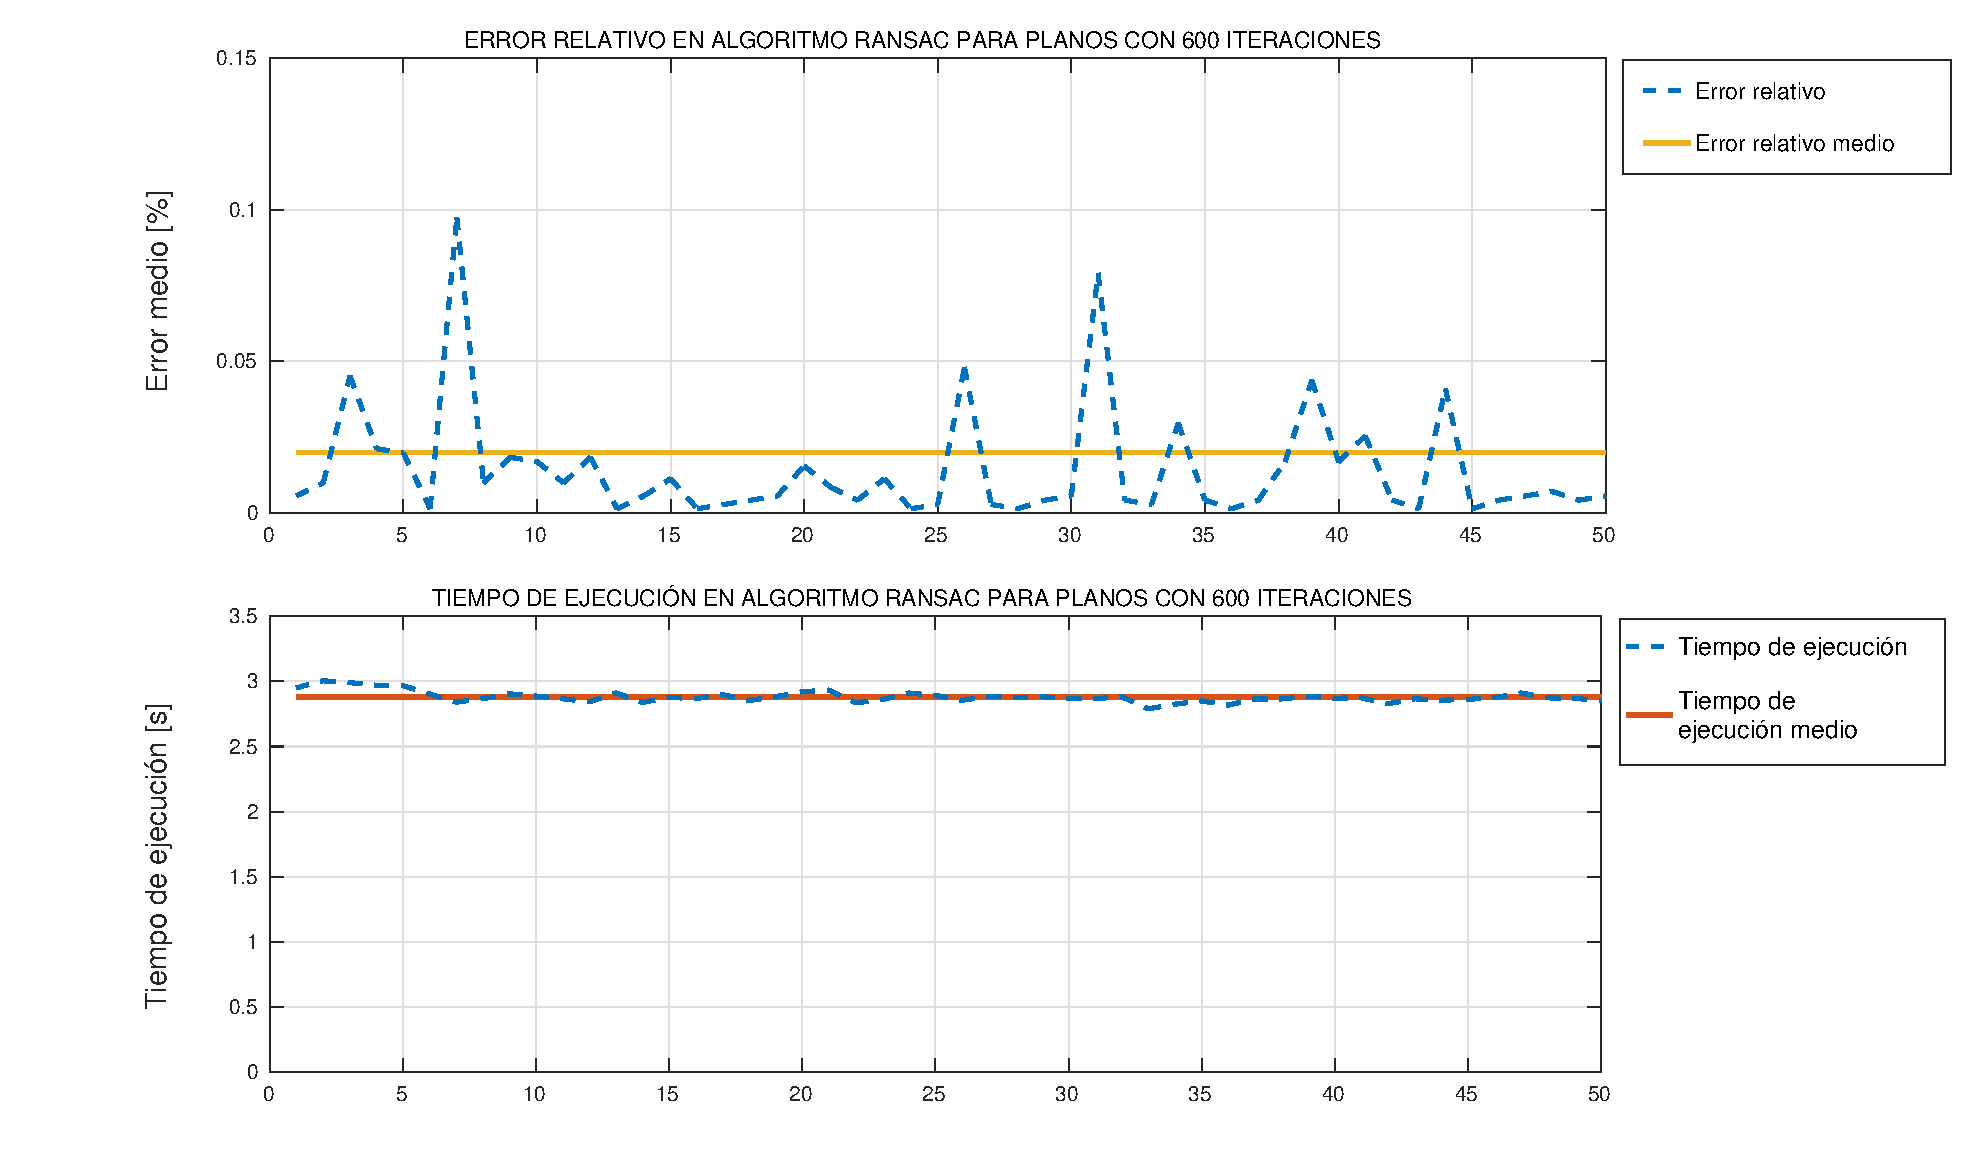
\includegraphics[width=16.0cm, height=9.0cm]{resultados/ransac_600}	
		\end{minipage}
		\begin{center}
		\caption{Gráfica correspondiente al error relativo para el algoritmo RANSAC para detección de planos con 600 iteraciones.}
		\end{center}
	\end{figure}
	
	\begin{figure}[H]
		\begin{minipage}{18cm}	
		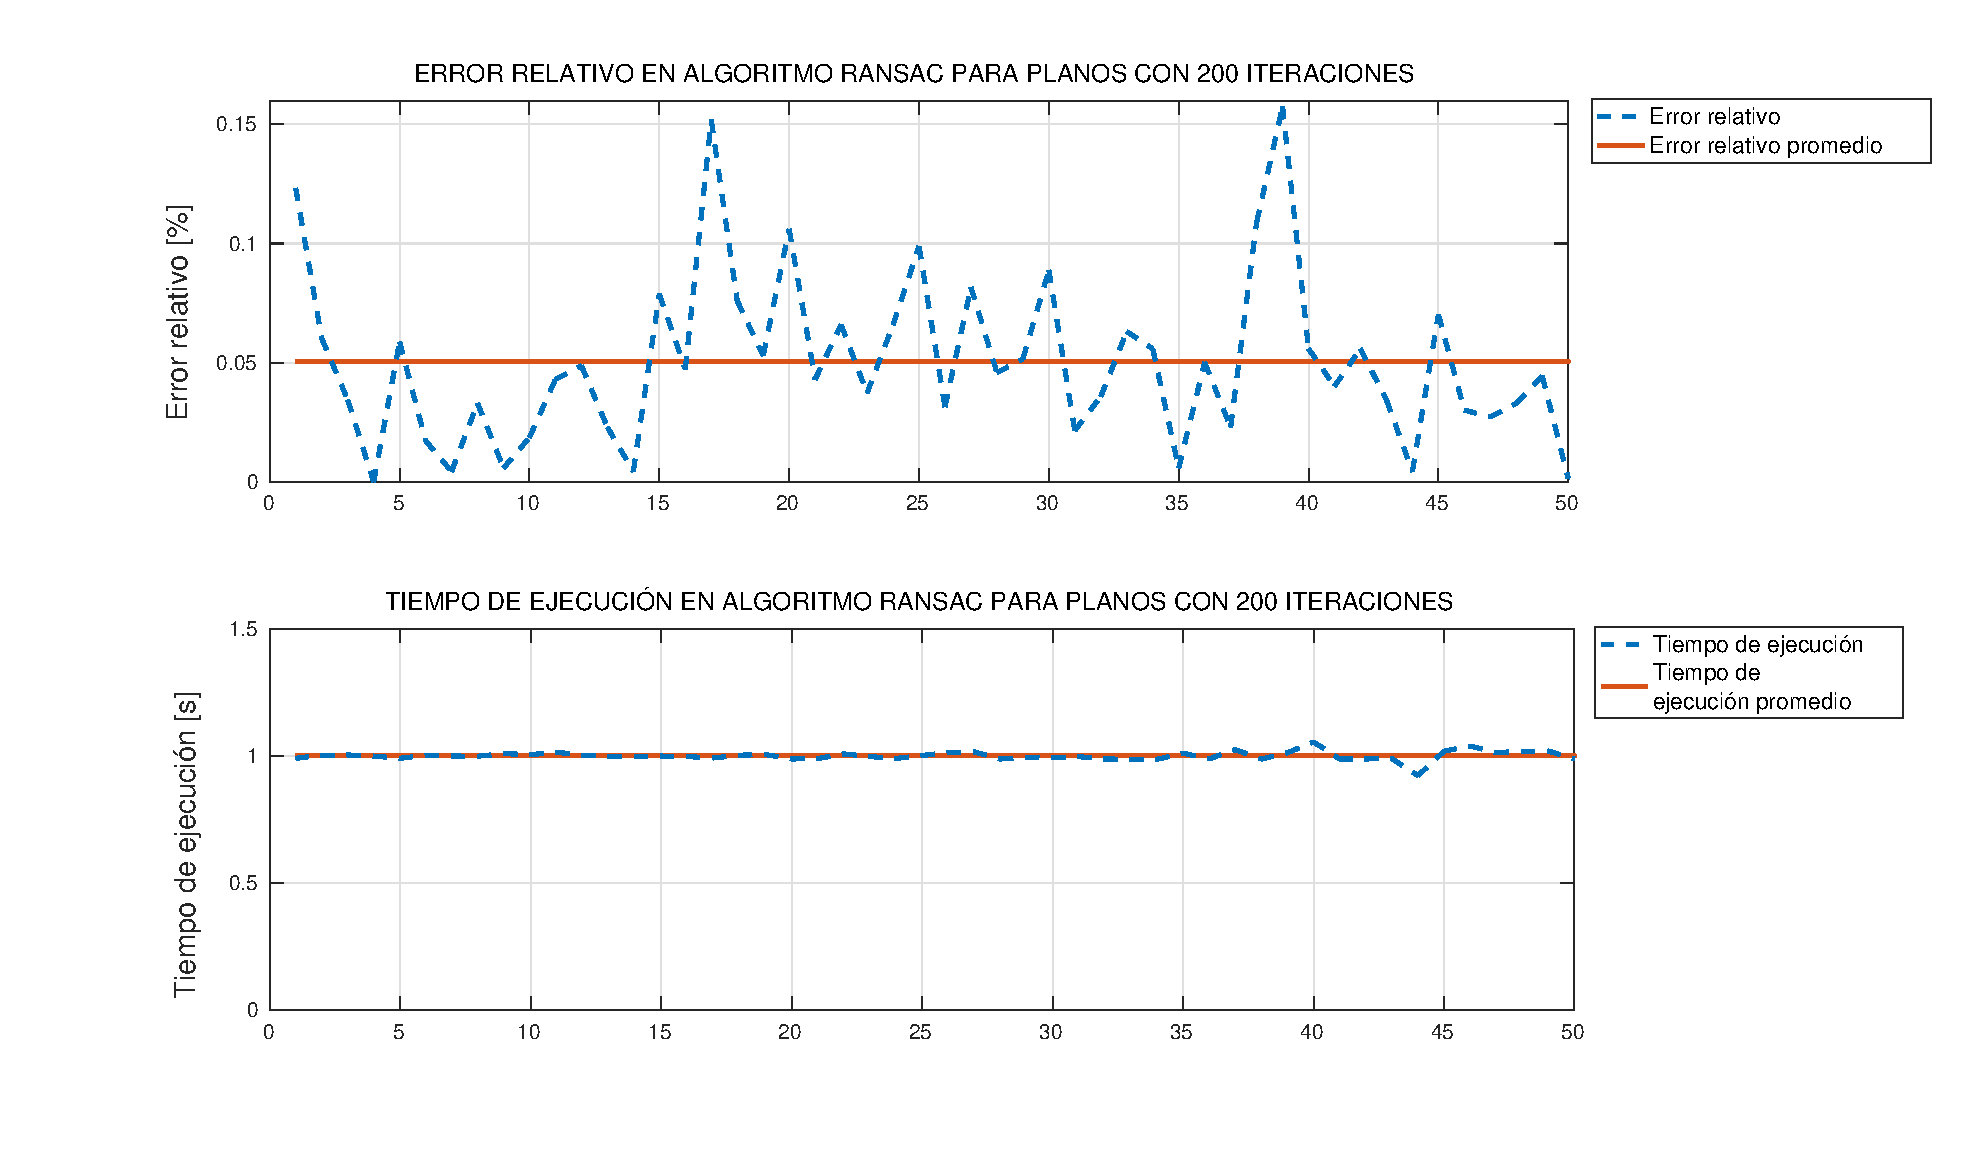
\includegraphics[width=16.0cm, height=9.0cm]{resultados/ransac_200}	
		\end{minipage}
		\begin{center}
		\caption{Gráficas correspondientes al error relativo y tiempo de ejecución para el algoritmo RANSAC con 200 iteraciones.}
		\end{center}
	\end{figure}

	\begin{figure}[H]
		\begin{minipage}{18cm}
		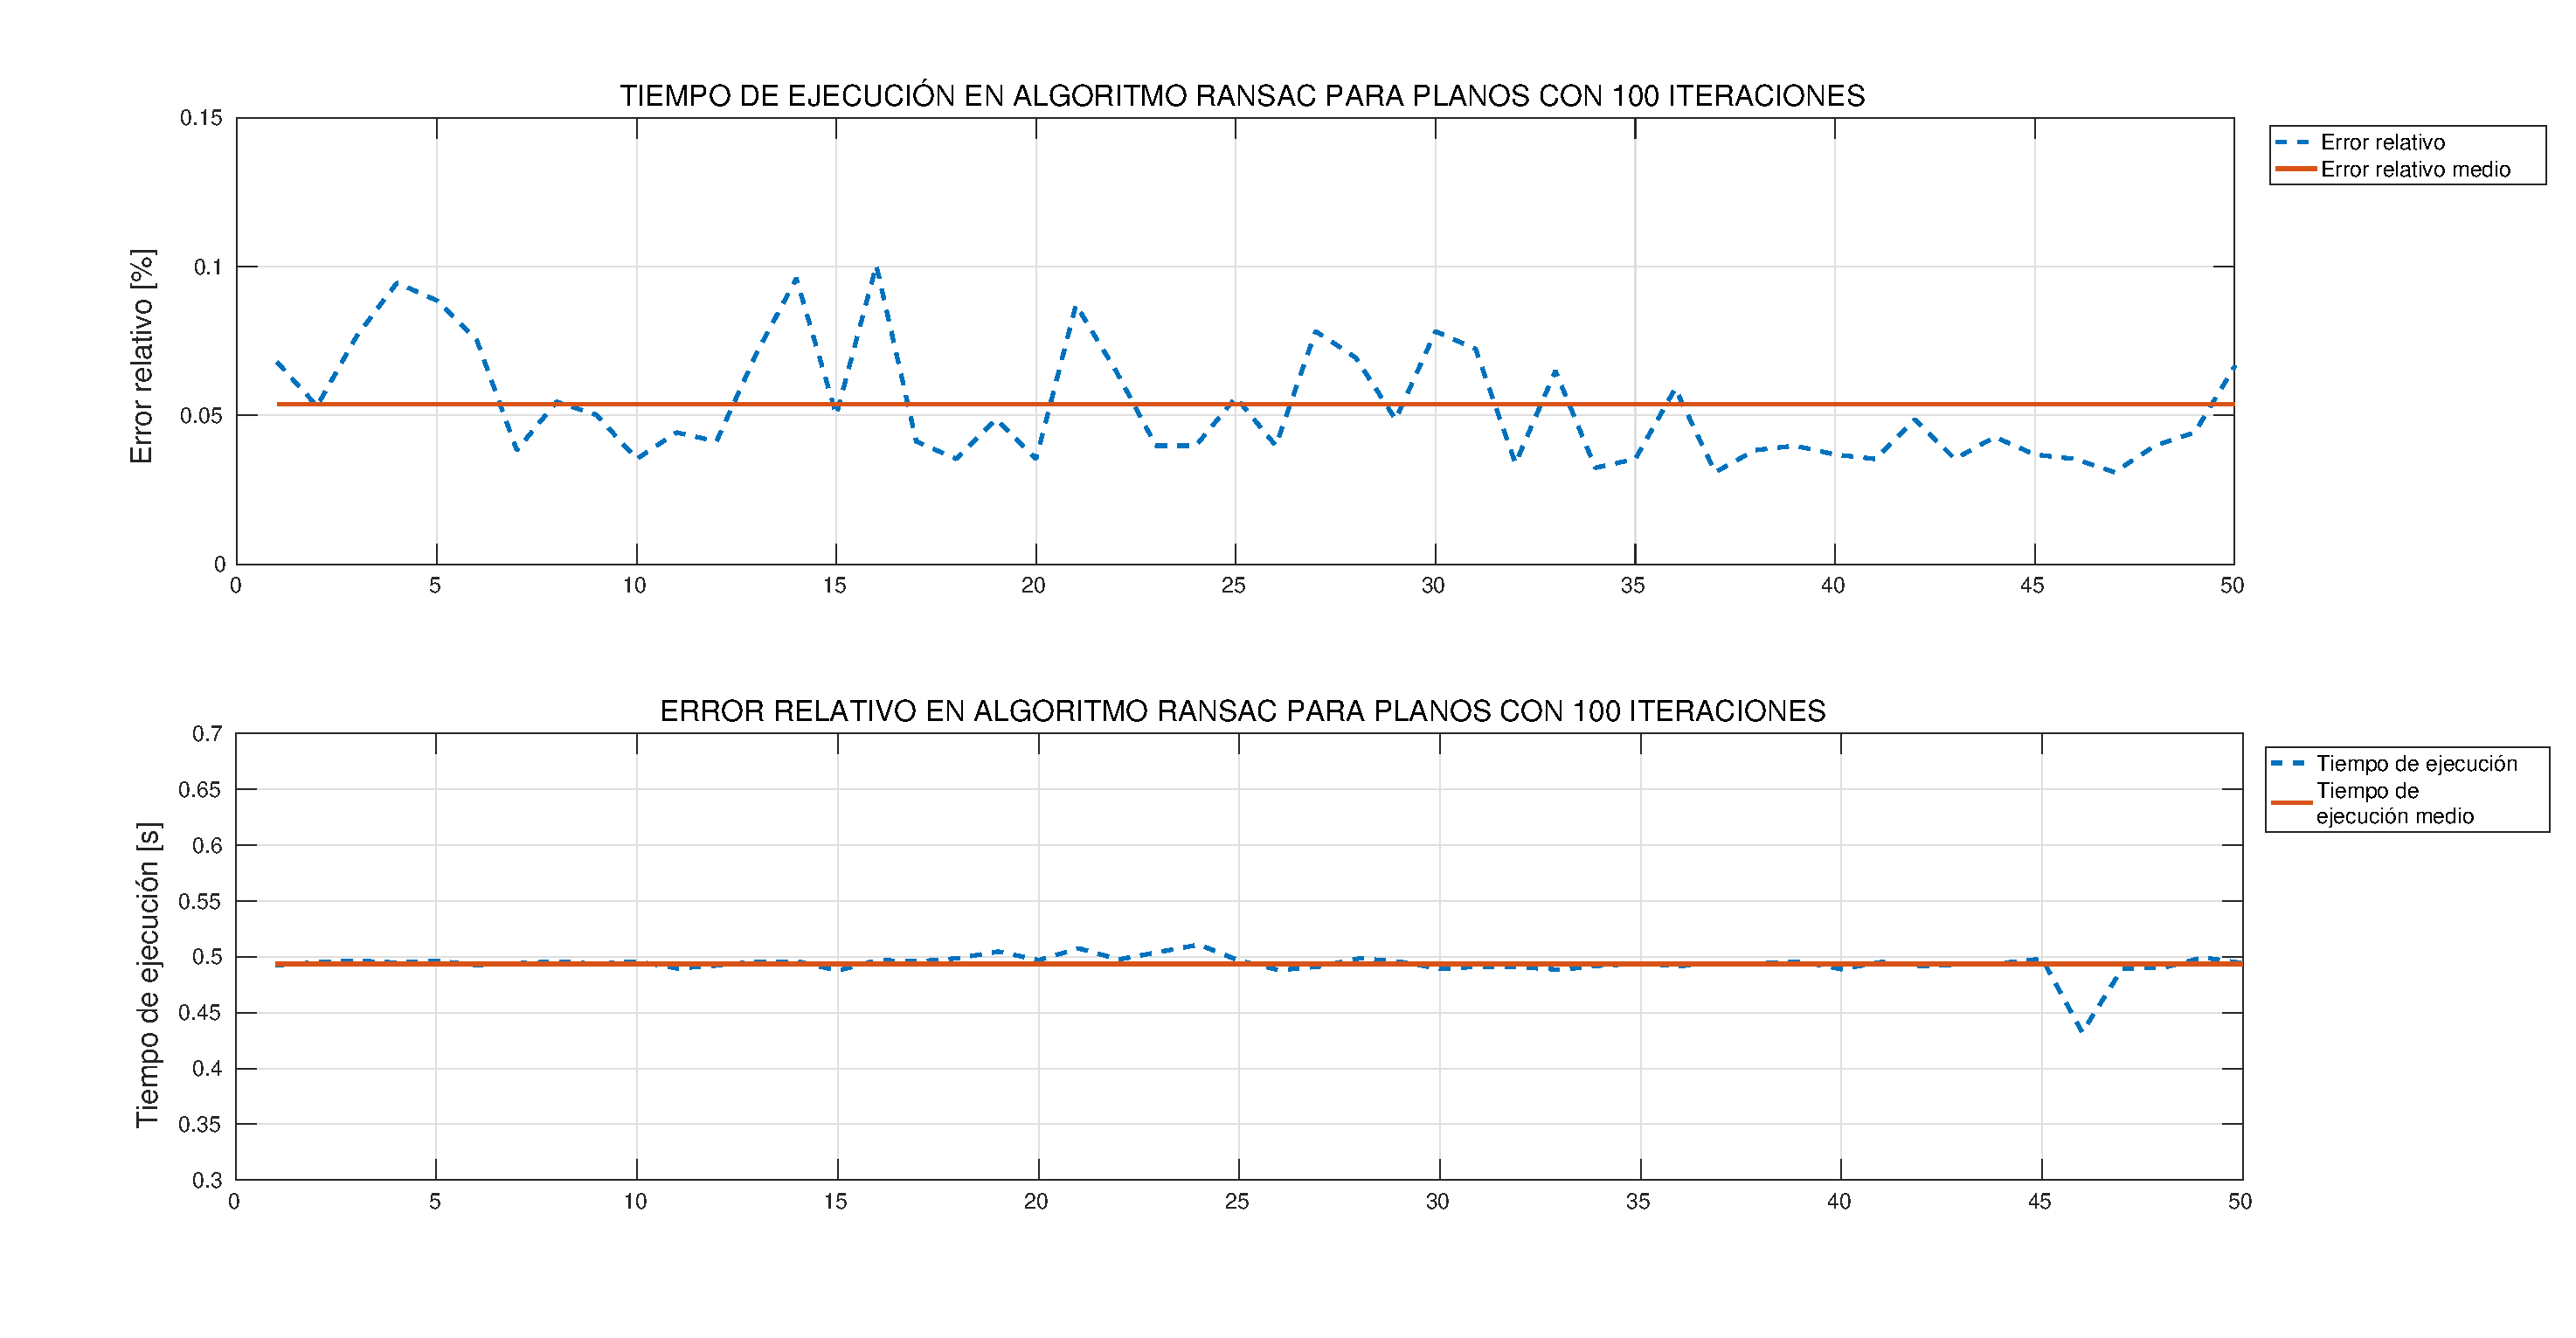
\includegraphics[width=16.0cm, height=9.0cm]{resultados/ransac_100_2}
		\end{minipage}
		\begin{center}
		\caption{Gráficas correspondientes al error relativo y tiempo de ejecución para el algoritmo RANSAC con 100 iteraciones.}
		\end{center}
	\end{figure}

	\begin{figure}[H]
		\begin{minipage}{18cm}
		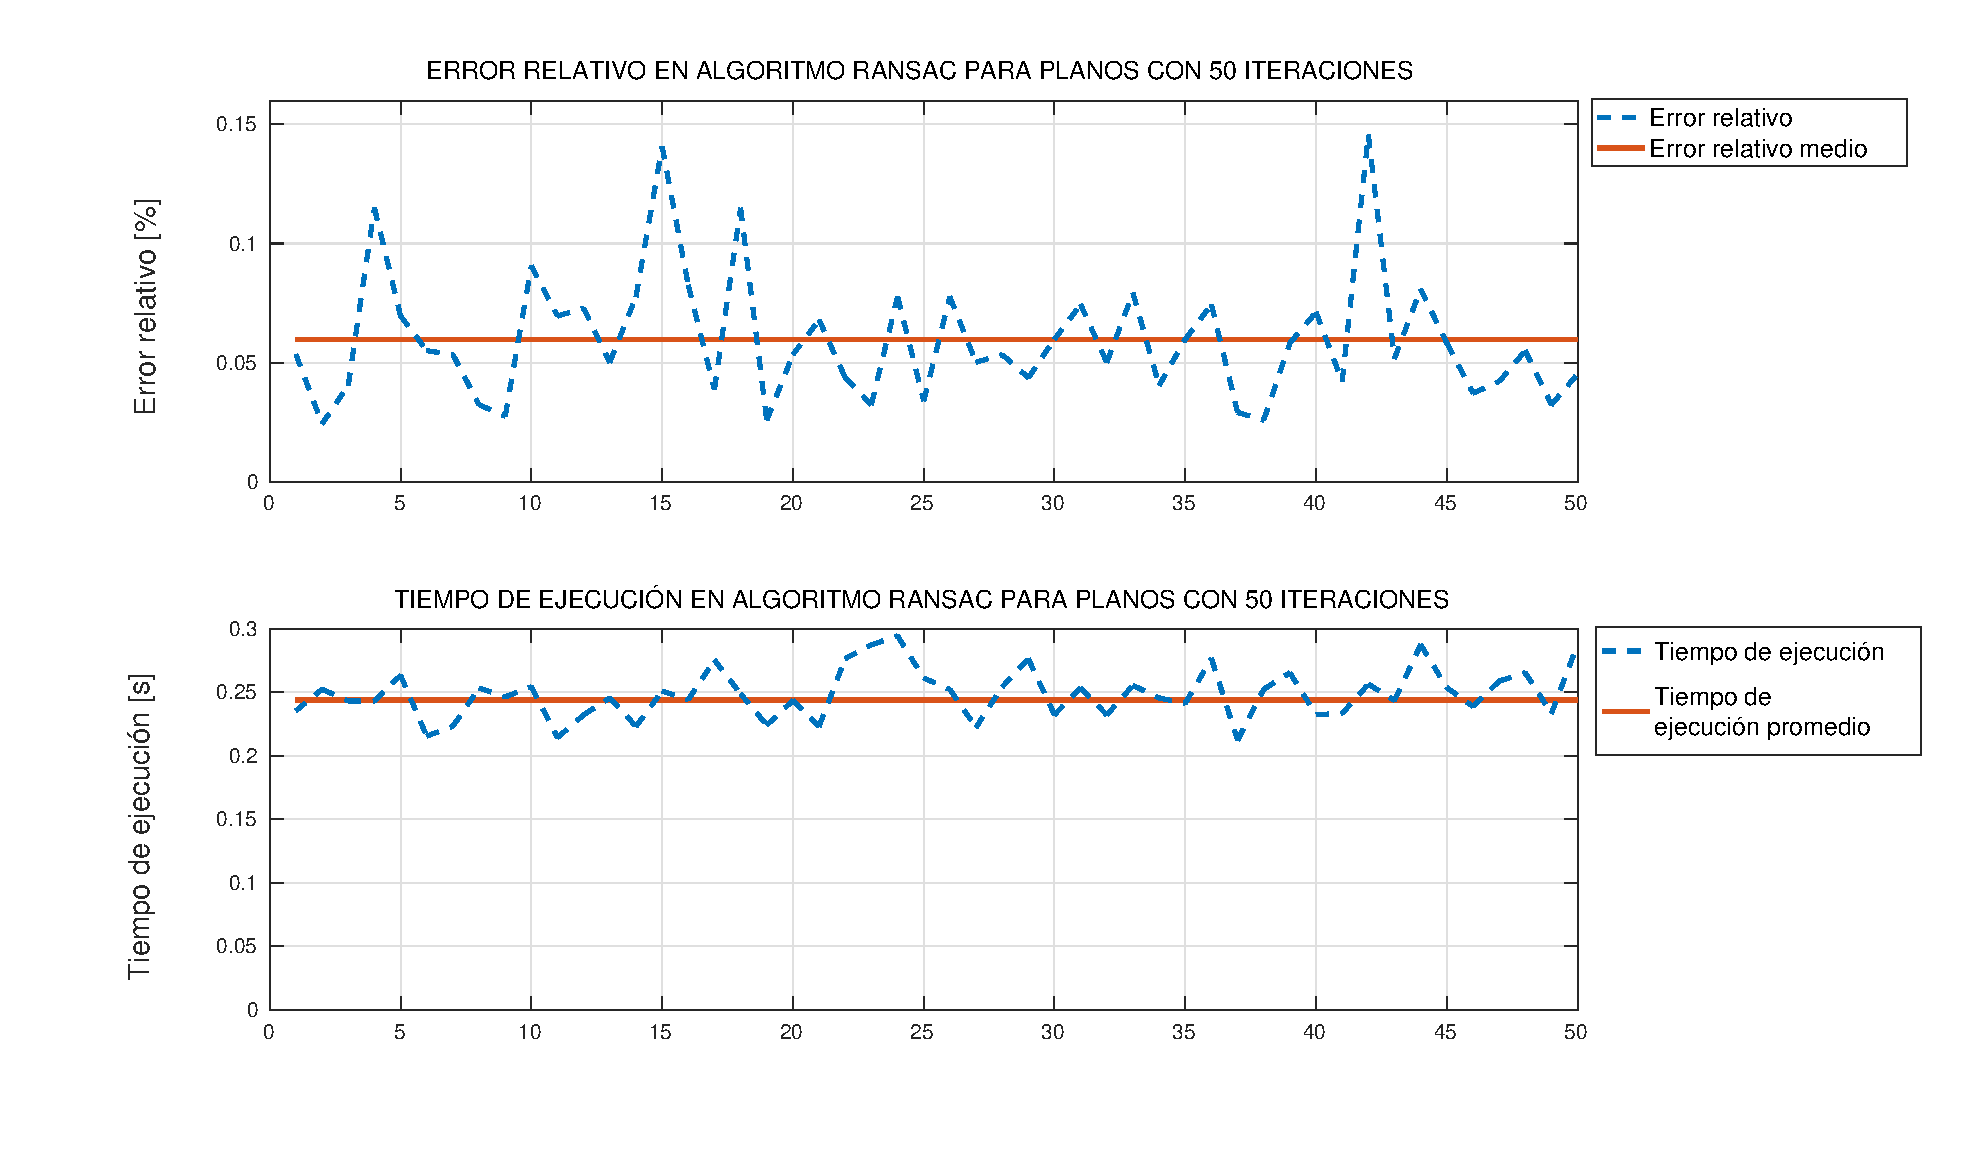
\includegraphics[width=16.0cm, height=9.0cm]{resultados/ransac_50}
		\end{minipage}
		\begin{center}
		\caption{Gráficas correspondientes al error relativo y tiempo de ejecución para el algoritmo RANSAC con 50 iteraciones.}
		\end{center}
	\end{figure}

	\begin{figure}[H]
		\begin{minipage}{18cm}
		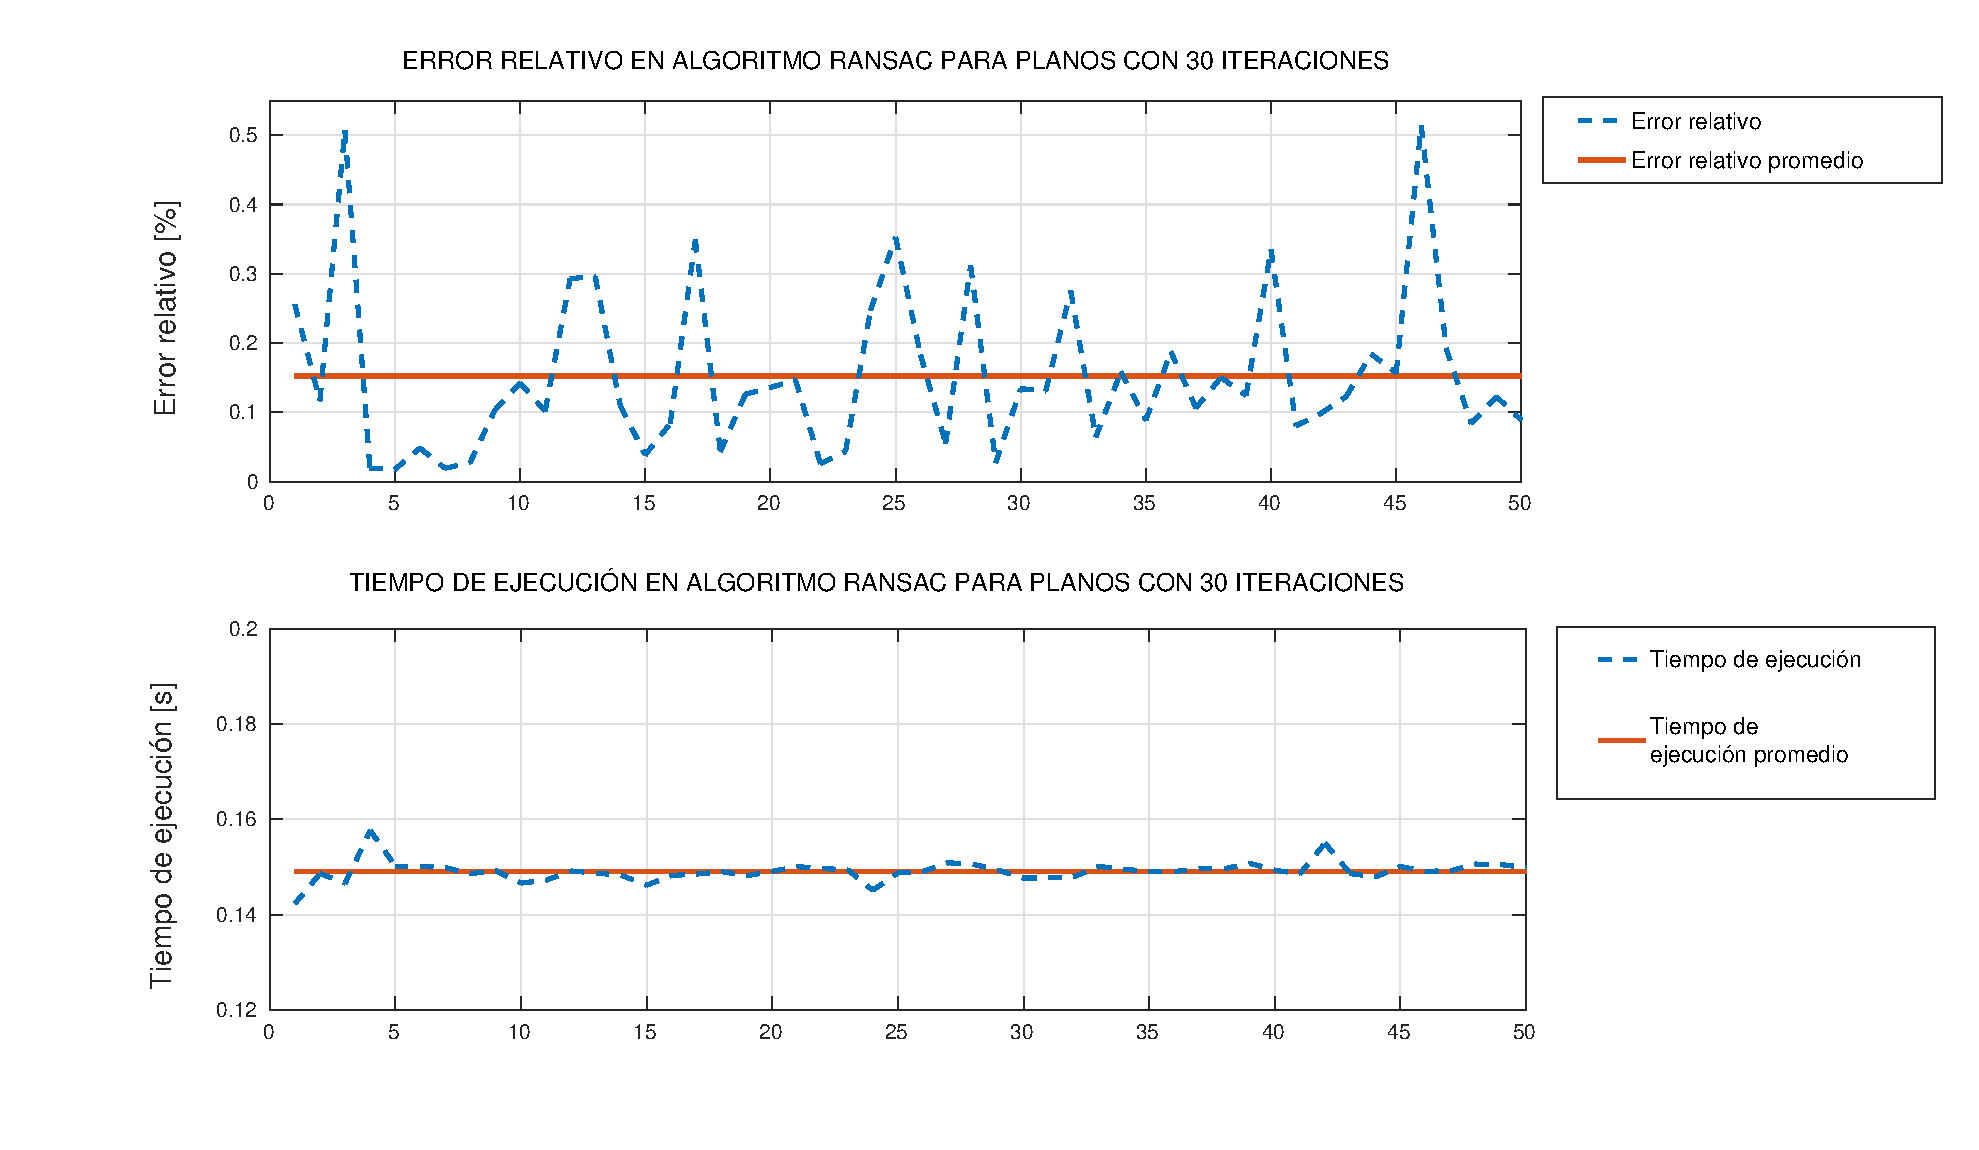
\includegraphics[width=16.0cm, height=9.0cm]{resultados/ransac_30}
		\end{minipage}
		\begin{center}
		\caption{Gráficas correspondientes al error relativo y tiempo de ejecución para el algoritmo RANSAC con 30 iteraciones.}
		\end{center}
	\end{figure}

	\begin{figure}[H]
		\begin{minipage}{18cm}
		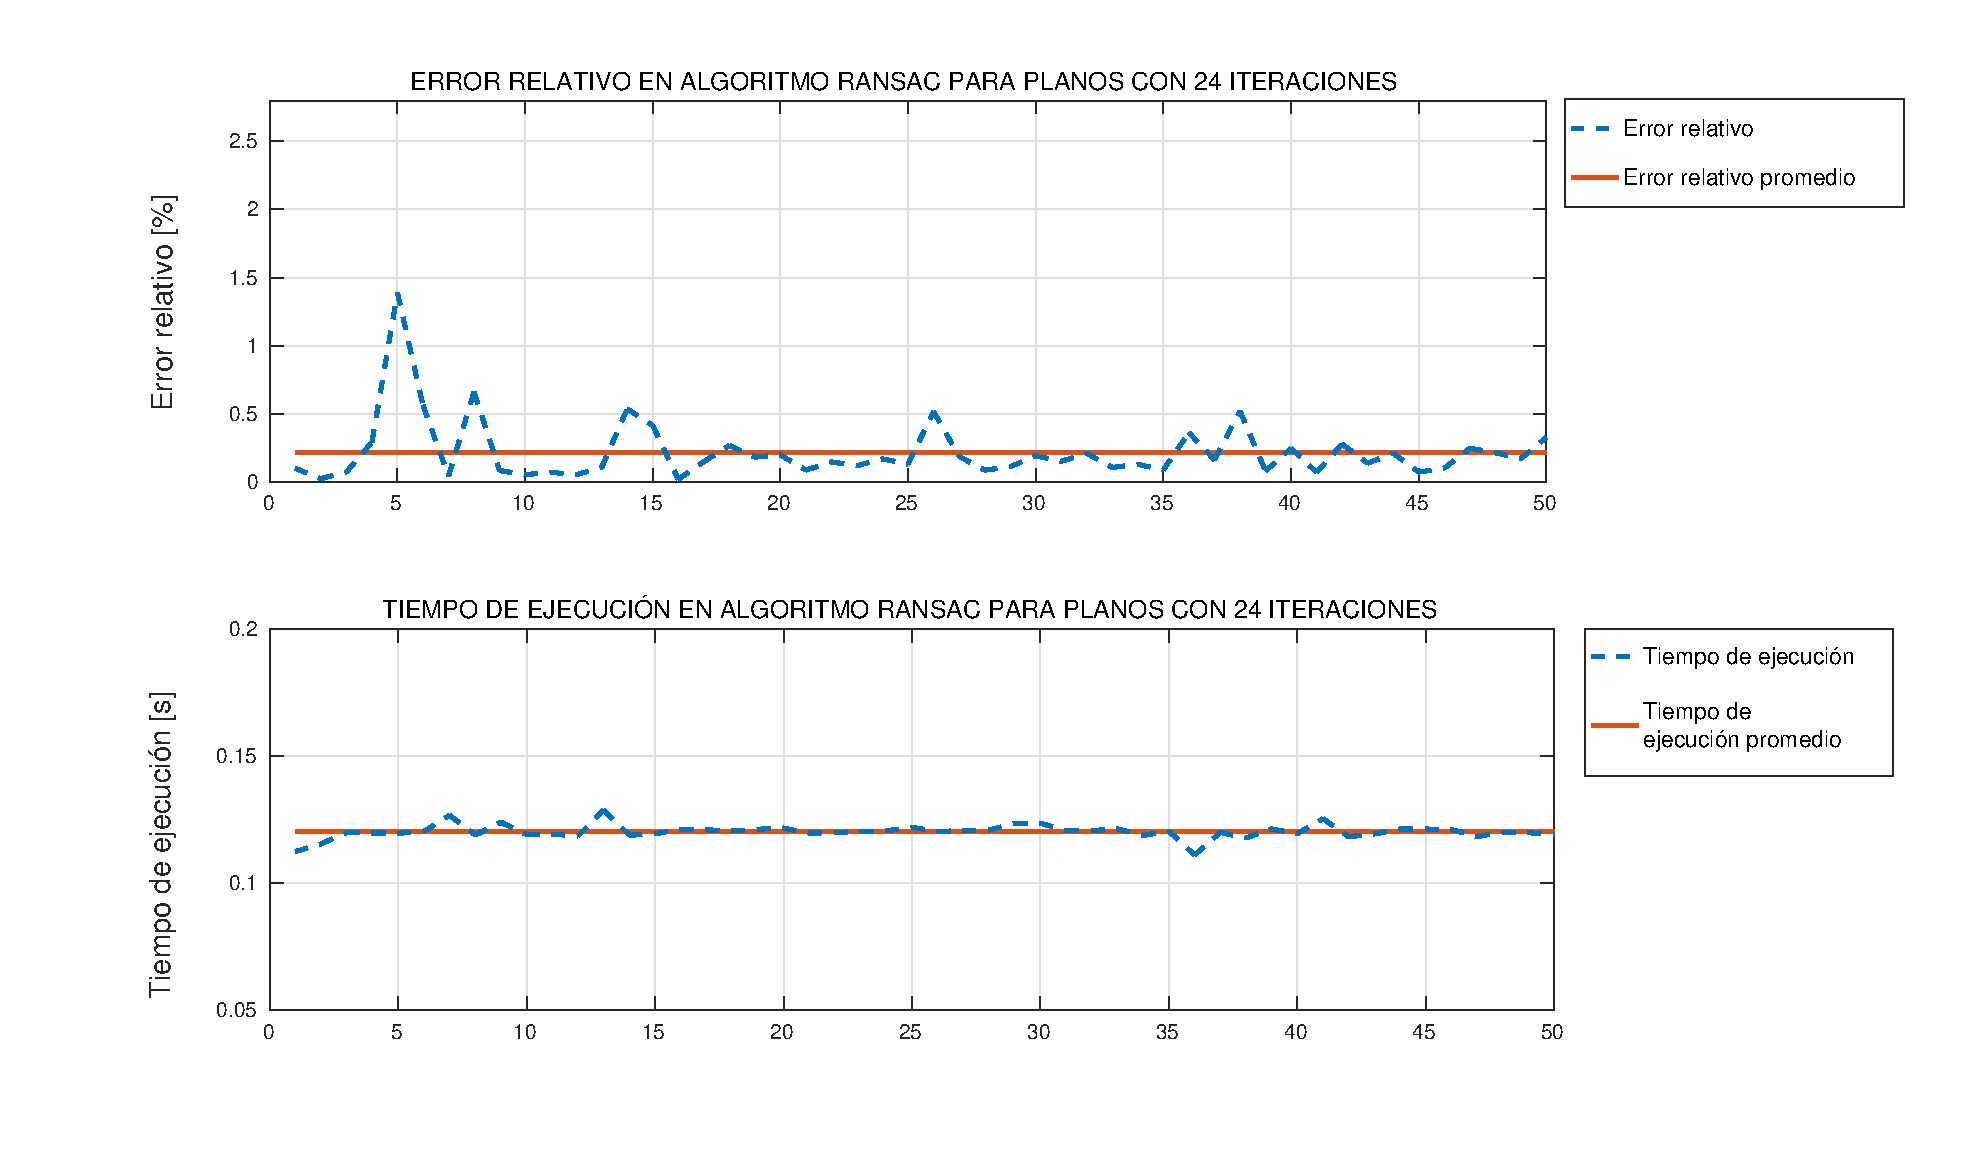
\includegraphics[width=16.0cm, height=9.0cm]{resultados/ransac_24}
		\end{minipage}
		\begin{center}
		\caption{Gráficas correspondientes al error relativo y tiempo de ejecución para el algoritmo RANSAC con 24 iteraciones.}
		\end{center}
	\end{figure}

	\begin{figure}[H]
		\begin{minipage}{18cm}	
		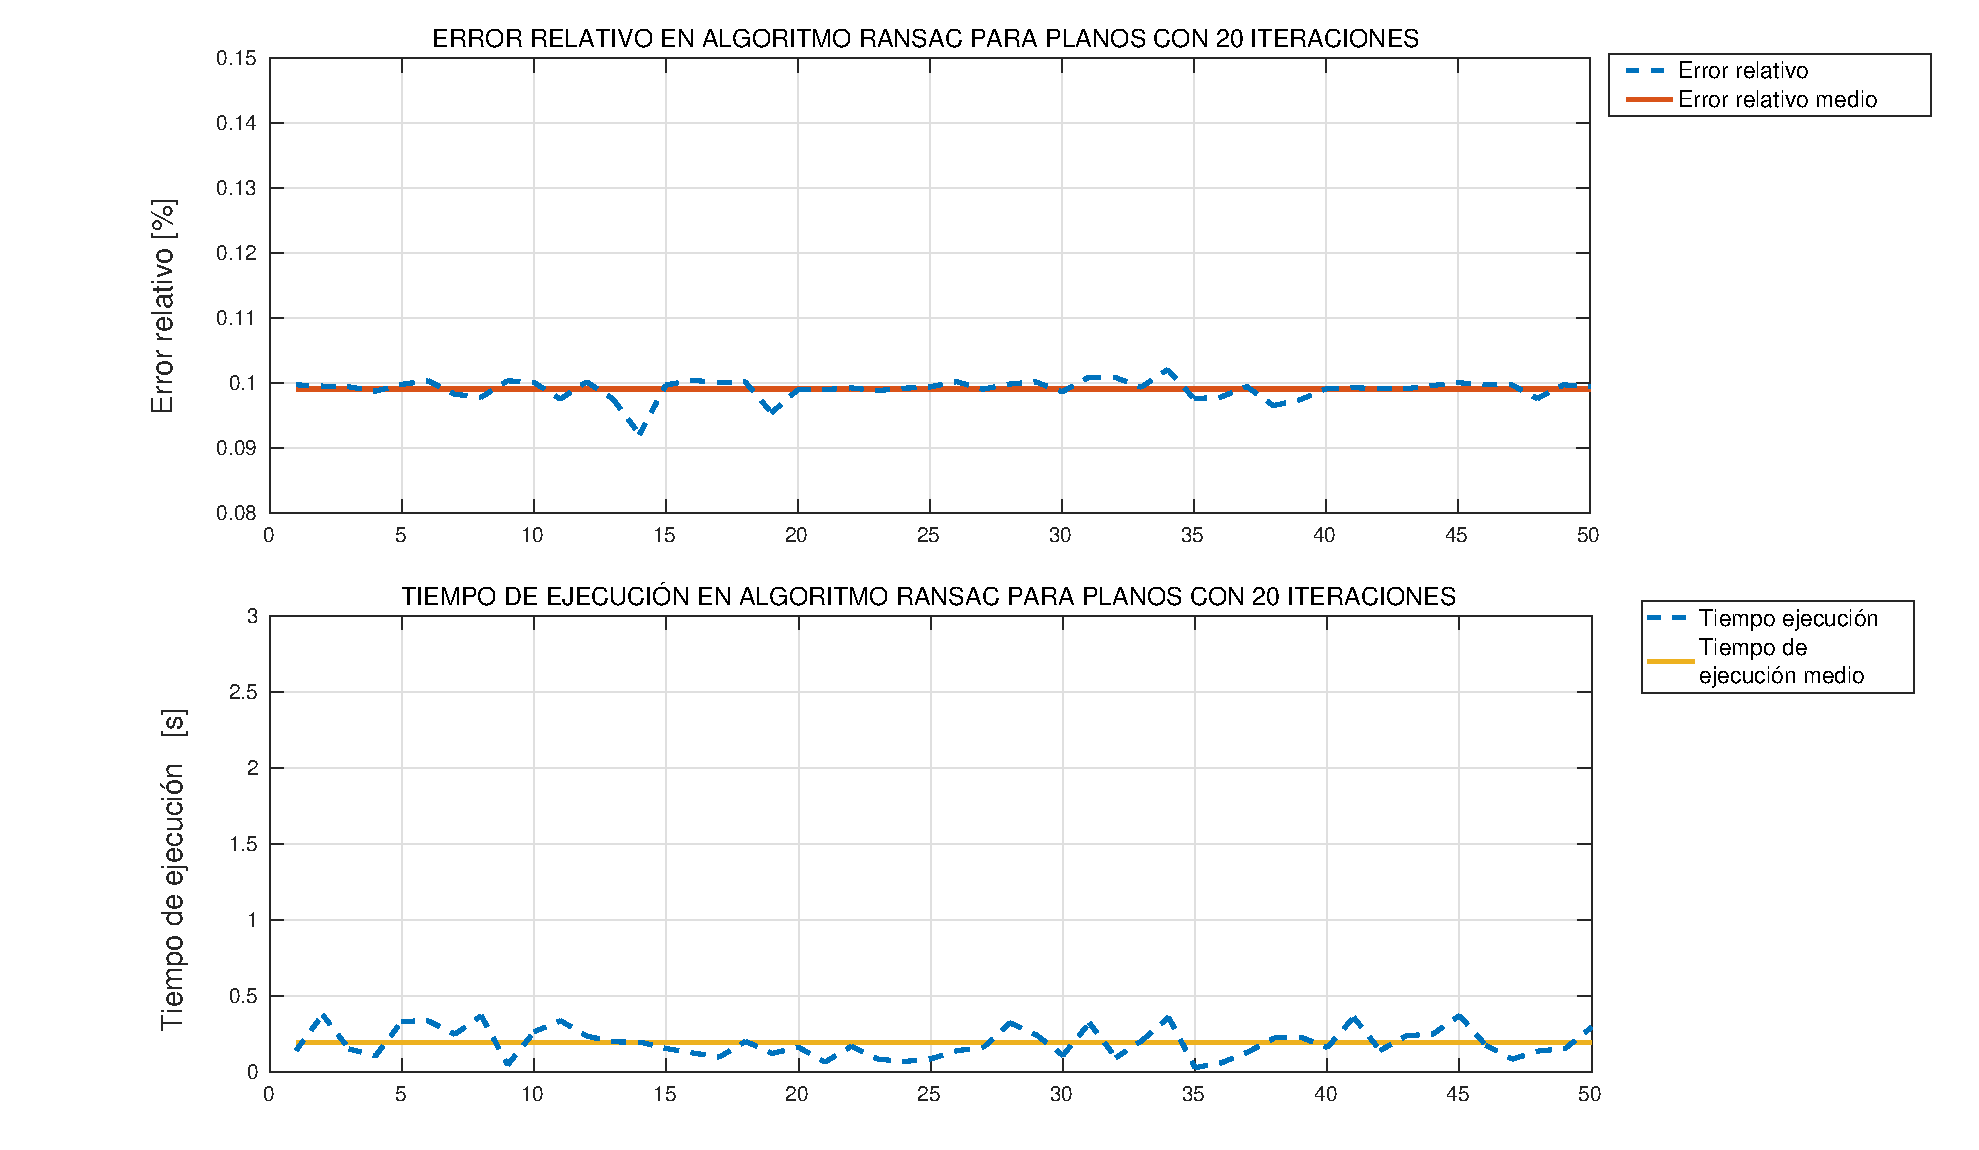
\includegraphics[width=16.0cm, height=9.0cm]{resultados/ransac_20}
		\end{minipage}
		\begin{center}
		\caption{Gráficas correspondientes al error relativo y tiempo de ejecución para el algoritmo RANSAC con 20 iteraciones.}
		\end{center}
	\end{figure}

	Una vez que se obtuvo la información parcial de cada uno de estos eventos se realizó una tabla extra que agrupa la información del tiempo de ejecución promedio y el error relativo promedio contra el número de iteraciones del algoritmo. Se obtuvo la siguiente gráfica.\\

	\begin{figure}[H]
		\begin{minipage}{18cm}
		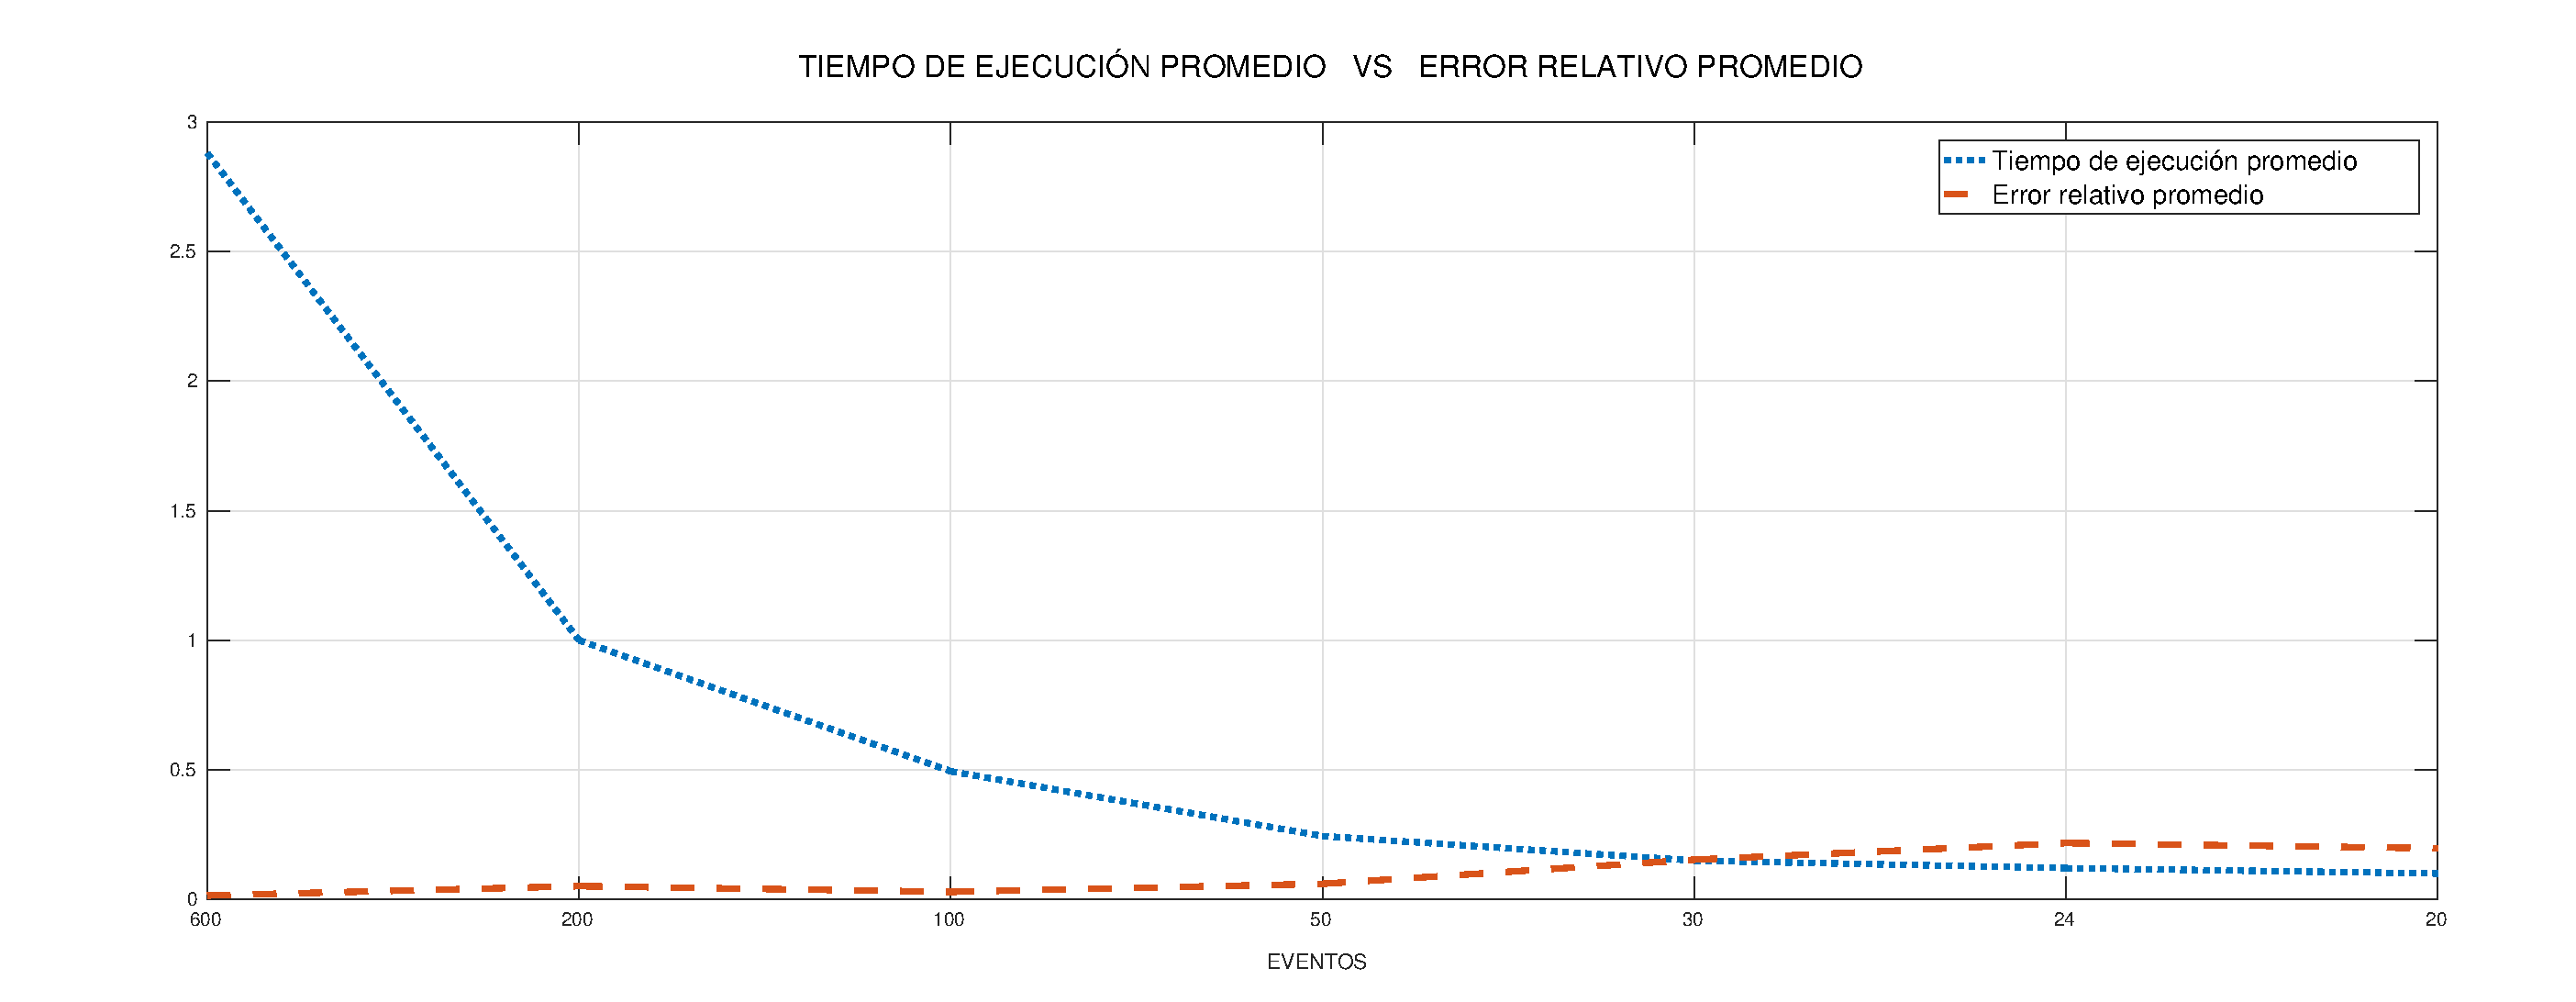
\includegraphics[width=16.0cm, height=12.0cm]{resultados/ransac_final}
		\end{minipage}

		\begin{center}
		\caption{Gráfica del error relativo vs tiempo de ejecución para diferentes números de iteraciones.}
		\label{Fig:RansacFinal}
		\end{center}
	\end{figure}


	Como podemos observar en la gráfica \ref{Fig:RansacFinal} el error relativo presenta un incremento conforme se disminuye el número de iteraciones en el algoritmo. El tiempo de ejecución por su parte muestra un decremento conforme número de iteraciones disminuye. Dado este comportamiento de ambos parámetros resulta difícil encontrar un punto de equilibrio entre estas dos unidades de medición. Para la aplicación particular de este trabajo se determinó un número óptimo de iteraciones entre 30 y 24.\\ 



	\subsection{Comparación exactitud y rapidez}
	Para este conjunto de pruebas se comparó el algoritmo desarrollado en el presente trabajo contra el implementado actualmente en el robot de servicio Justina, reportado en el trabajo de tesis \cite{cruz2016detection}.\\

	Las pruebas se desarrollaron de la siguiente manera, con la estructura de comunicación que permite ROS se implementaron dos servicios para encontrar planos: el desarrollado en este trabajo de tesis y el algoritmo ya implementado. Se obtuvo la información de profundidad con el sensor RGB-D Kinect, esta información se compartió a través de un tópico al cual ambos servicios se encontraban suscritos. De esta manera nos aseguramos de contar con la misma información en ambos algoritmos para poner a prueba la velocidad de ejecución y la precisión de algoritmo.\\


	En cuanto a la medida de precisión del algoritmo continuamos suponiendo un plano horizontal del cual conocemos su altura; por tanto podemos conocer la ecuación del plano horizontal a esa altura. Se puso a prueba el algoritmo para ese modelo y se observó la cantidad de puntos que entran en ese modelo, tomando este resultado como el ideal. Posteriormente se pusieron en funcionamiento ambos algoritmos midiendo la cantidad de puntos en los modelos obtenidos y comparándolos con el número de puntos ideal. Este evento se iteró 80 veces.\\


	Posteriormente se calculó el error relativo entre el modelo ideal y cada uno de los algoritmos como se muestra en la tabla \ref{t_result:1} la cual resume los resultados obtenidos durante las pruebas.\\

	\begin{table}[h!]
	\centering 
	\begin{tabular}{ |p{6.5cm}||p{2.1cm}|p{2.1cm}|  }
	 \hline
	 \multicolumn{3}{|c|}{ Resultados algoritmo RANSAC } \\
	 \hline
	 \multicolumn{3}{|c|}{ Número de iteraciones: 1000}\\
	 \hline
	 \multicolumn{3}{|c|}{ Distancia miníma al modelo: 0.02[m]}\\
	 \hline
	                               &  Anterior     &	Propuesto \\
	 \hline
	 Tiempo promedio de ejecución  &  96.24[ms]    &   701.5[ms]\\
	 \hline
	 Error relativo promedio       &  39.95        &    8.78\\
	 \hline
	\end{tabular}
	\caption{Comparación de resultados de RANSAC para planos.}
	\label{t_result:1}
	\end{table}


	Con la información de la tabla \ref{t_result:1} se puede deducir que la nueva implementación del algoritmo RANSAC con 1000 iteraciones y una distancia mínima al modelo de 0.02[m] es más lenta pero con menor error relativo. La diferencia de 605[ms] puede llegar a ser significativa si se requiere ejecutar el algoritmo iterativamente, sin embargo, el común de las pruebas en robots de servicio doméstico no suelen requerir este tipo de acciones.\\  





\newpage
%%%%%%%%%%%%%%%%%%%%%%%%%%%%%%%%%%%%%%%%%%%%%%%%%%%%%%%%%%%%%%%%%%%%
%%%%%%%%%     CARACTERISTICAS OBJETOS          %%%%%%%%%%%%%%%%%%%%%
	\section{Extracción de objetos y sus características}
	En lo que respecta a la extracción de objetos y sus características se realizó una caracterización de la misma. Para ello se realizaron un total de 100 eventos para cada uno de los 5 objetos diferentes: un control para videojuegos de forma irregular, una caja de cereal, un envase de jugo, un envase de bebida láctea y una barra de chocolate. Como información de interés se compararon las medidas de altura de los objetos. Puesto que el algoritmo previo también hacía una estimación de la altura de los objetos se compararon los resultados de ambos algoritmos.\\

	\begin{figure}[H]
		\centering
		\includegraphics[scale=0.06]{objs_real/objects_2.jpg}	
		\caption{Fotografía de los objetos utilizados en las pruebas de cálculo de alturas y de manipulación de objetos.}
		\label{fig:objectsComplete}
	\end{figure}


	\subsection{Estimación de alturas}

	\begin{figure}[H]
		\begin{subfigure}[h]{.30\textwidth}
		\includegraphics[scale=0.04]{objs_real/cerealBoxHeight.jpg}	
		\end{subfigure}%
		\begin{subfigure}[h]{.5\textwidth}
		\includegraphics[scale=0.40]{resultados/cerealAltura_media.png}	
		\end{subfigure}
		\caption*{(a)}
		\label{fig:mesh1}
	\end{figure}

	\begin{figure}[H]
		\begin{subfigure}[h]{.30\textwidth}
		\includegraphics[scale=0.04]{objs_real/jugoHeight.jpg}	
		\end{subfigure}%
		\begin{subfigure}[h]{.5\textwidth}
		\includegraphics[scale=0.40]{resultados/jugoAltura_media.png}	
		\end{subfigure}
		\caption*{(b)}
		\label{fig:mesh1}
	\end{figure}

	\begin{figure}[H]
		\begin{subfigure}[h]{.30\textwidth}
		\includegraphics[scale=0.06]{objs_real/milkHeight.jpg}	
		\end{subfigure}%
		\begin{subfigure}[h]{.5\textwidth}
		\includegraphics[scale=0.40]{resultados/lecheAltura_media.png}	
		\end{subfigure}
		\caption*{(c)}
		\label{fig:mesh1}
	\end{figure}

	\begin{figure}[H]
		\begin{subfigure}[h]{.30\textwidth}
		\includegraphics[scale=0.04]{objs_real/joystickHeight2.jpg}	
		\end{subfigure}%
		\begin{subfigure}[h]{.5\textwidth}
		\includegraphics[scale=0.40]{resultados/joystickAltura_media.png}	
		\end{subfigure}
		\caption*{(d)}
		\label{fig:mesh1}
	\end{figure}

	\begin{figure}[H]
		\begin{subfigure}[h]{.30\textwidth}
		\includegraphics[scale=0.04]{objs_real/chocolateHeight2.jpg}	
		\end{subfigure}%
		\begin{subfigure}[h]{.5\textwidth}
		\includegraphics[scale=0.40]{resultados/chocolateAltura_media.png}	
		\caption*{(e)}
		\end{subfigure}
		\caption{Gráficas de alturas para: (a) una caja de cereal, (b) una caja de jugo, (c) un envase de leche, (d) un control de videojuegos, (e) una barra de chocolate. \\La altura real del objeto (amarillo), la altura estimada con el algoritmo previo (rojo) y la estimación actual (azul).}
		\label{fig:mesh1}
	\end{figure}

	Posteriormente, se realizó una prueba T para muestras pareadas (prueba t de mediciones repetidas) con el objetivo de saber si son significativamente diferentes. En el caso de este trabajo es necesario saber si las medias de las muestras tomadas realmente representan una mejor estimación de alturas.\\

	A continuación se reportan los valores de medias, con el valor T obtenido para cada conjunto de pruebas y el valor de significancia para comparar altura estimada por algoritmo previo vs altura estimada por algoritmo actual.\\

\begin{table}[H]
	\centering
	\begin{tabular}{ |p{2.0cm}|p{2.0cm}|p{2.0cm}|p{2.0cm}|p{2.0cm}|p{2.0cm}|p{2.0cm}|  }
	 \hline
	 & \multicolumn{2}{|c|}{\textbf{Algoritmo previo} } & \multicolumn{2}{|c|}{\textbf{Algoritmo actual}} &  &\\
	 \hline
	 \textbf{Objeto} &\textbf{Altura media [m]}  &\textbf{Varianza}&\textbf{Altura media [m]}  &\textbf{Varianza} &\textbf{$T_{value}$} & \textbf{$P_{value}$}\\
	 \hline
	  Cereal    &	 0.2568  & $1.79e^{-6}$ & 0.2324 & $4.22e^{-6}$ & -26.77 & $p_{value} < 2.2e^{-16}$  \\
	 \hline
	  Jugo      &    0.1407  & $3.28e^{-6}$ & 0.1305 & $1.67e^{-6}$ & -64.854 & $p_{value} < 2.1e^{-16}$  \\
	 \hline
	  Leche     &    0.0901  & $7.33e^{-6}$ & 0.0889 & $5.54e^{-6}$ & 1.8081 & $p_{value} < 2.1e^{-16}$  \\
	 \hline 
	  Control de videojuegos &  0.0485  & $6.28e^{-6}$ &0.0411 & $7.01e^{-6}$ & 1.3817 & $p_{value} = 0.0175$ \\
	 \hline
	  Barra de chocolate   &    0.0215  & $3.3e^{-6}$  &0.0213 & $4.4e^{-6}$ & -11.42 & $p_{value} = 0.1335$ \\
	 \hline
	\end{tabular}
	\caption{Tabla de resultados de la prueba T a medidas repetidas para la altura de 5 objetos.}
	\label{t_test:alturas}
\end{table}




\newpage
%%%%%%%%%%%%%%%%%%%%%%%%%%%%%%%%%%%%%%%%%%%%%%%%%%%%%%%%%%%%
%%%%%%%%% Cálculo de las orientaciones  %%%%%%%%%%%%%%%%%%%%
	\section{Cálculo de la orientación del objeto.}

	En esta sección del trabajo se reportan los resultados obtenidos al realizar las pruebas de estimación de orientación de los objetos sobre un plano. En esta prueba se realizaron 50 tomas de datos para cada uno de los objetos con diferentes orientaciones.\\

	El proceso para poner a prueba la estimación de ángulos de los objetos con respecto del eje Y del robot se describe a continuación. Una vez obtenidos los vectores propios de la matriz de covarianzas, se obtiene un conjunto de vectores ortogonales que nos indican los ejes en los cuales sucede la mayor distribución de puntos de un objeto. Con este conjunto de vectores se realizaron dos procesos:\\

	\begin{itemize}
		\itemsep -0.08in
		\item{Un ordenamiento por magnitud.}
		\item{Una ordenamiento por magnitudes en las respectivas componentes $x, y, z$}
	\end{itemize}  

		Con la información de los vectores ordenados se puede comparar si el mayor eje de distribución ocurre en el eje $z$ del robot o si ocurre en alguno de los vectores paralelos al conjunto de vectores que definirían el plano sobre el cual se encuentran los objetos.\\

		El algoritmo para calcular el ángulo del objeto con respecto del eje $z$ del robot, se explica de la siguiente manera: se toma el vector paralelo al plano con mayor magnitud, puesto que sabemos del ordenamiento cual es el vector con una componente mayor en el eje $z$ lo descartamos del proceso, con los dos vectores restantes obtenemos el de mayor magnitud.\\

		Este vector apuntaría en la dirección $y$ o $-y$ para un caso ideal en que el ángulo del objeto fuera de cero grados medido sobre el eje $z$ del robot. en este punto se realiza un acotamiento para que dicho vector quede en el primer y segundo cuadrante de un sistema coordenado, posteriormente se calcula el ángulo de rotación por medio del producto punto que existe entre el ángulo del vector estimado para el objeto y el vector que apunta en la dirección del vector unitario $y$ del robot.\\


		%\newpage
		\subsection{Pruebas para objetos a 0 grados}

		Los resultados que se obtuvieron de la prueba antes mencionada, se muestran en las siguientes gráficas.\\ 

		\begin{figure}[H]
			\begin{subfigure}[h]{.30\textwidth}
			\includegraphics[scale=0.30]{objs_real/cereal_0Degrees}	
			\end{subfigure}%
			\begin{subfigure}[h]{.5\textwidth}
			\includegraphics[scale=0.40]{resultados/angulos_cereal}	
			\caption*{(a)}
			\end{subfigure}
		\end{figure}

		\begin{figure}[H]
			\begin{subfigure}[h]{.30\textwidth}
			\includegraphics[scale=0.30]{objs_real/juice_0Degrees}
			\end{subfigure}%
			\begin{subfigure}[h]{.5\textwidth}
			\includegraphics[scale=0.40]{resultados/angulos_jugo.png}
			\caption*{(b)}
			\end{subfigure}
		\end{figure}

		\begin{figure}[H]
			\begin{subfigure}[h]{.30\textwidth}
			\includegraphics[scale=0.30]{objs_real/milk_0Degrees}
			\end{subfigure}%
			\begin{subfigure}[h]{.5\textwidth}
			\includegraphics[scale=0.40]{resultados/angulos_milk.png}
			\caption*{(c)}
			\end{subfigure}
		\end{figure}

		\begin{figure}[H]
			\begin{subfigure}[h]{.30\textwidth}
			\includegraphics[scale=0.30]{objs_real/joystick_0Degrees}
			\end{subfigure}%
			\begin{subfigure}[h]{.5\textwidth}
			\includegraphics[scale=0.40]{resultados/angulos_joystick.png}
			\caption*{(d)}
			\end{subfigure}
		\end{figure}

		\begin{figure}[H]
			\begin{subfigure}[h]{.30\textwidth}
			\includegraphics[scale=0.25]{objs_real/chocolate_0Degrees}
			\end{subfigure}%
			\begin{subfigure}[h]{.5\textwidth}
			\includegraphics[scale=0.40]{resultados/angulos_chocolate.png}
			\caption*{(e)}
			\end{subfigure}
			\caption{Gráficas de estimaciones de ángulos para: (a) caja de cereal,  (b) caja de jugo, (c) envase de leche, (d) control de videojuegos, (e) una barra de chocolate con orientación de 0 grados respecto al eje $y$ del robot.}
		\end{figure}



		\newpage
		%%%%%%%%%%%%%%%%%%%%%%%%%%%%%%%%%%%%%%%%%%%%%%%%%%%%%%%%%%%%%%%%%
		% PRUEBAS A 45 GRADOS %
		\subsection{Pruebas para objetos a 45 grados}

		\begin{figure}[H]
			\begin{subfigure}[h]{.30\textwidth}
			\includegraphics[scale=0.30]{objs_real/cereal_45Degrees}	
			\end{subfigure}%
			\begin{subfigure}[h]{.5\textwidth}
			\includegraphics[scale=0.40]{resultados/angulos_cereal_45.png}	
			\caption*{(a)}
			\end{subfigure}
		\end{figure}

		\begin{figure}[H]
			\begin{subfigure}[h]{.30\textwidth}
			\includegraphics[scale=0.30]{objs_real/juice_45Degrees}
			\end{subfigure}%
			\begin{subfigure}[h]{.5\textwidth}
			\includegraphics[scale=0.40]{resultados/angulos_jugo_45.png}
			\caption*{(b)}
			\end{subfigure}
		\end{figure}

		\begin{figure}[H]
			\begin{subfigure}[h]{.30\textwidth}
			\includegraphics[scale=0.30]{objs_real/milk_45Degrees}
			\end{subfigure}%
			\begin{subfigure}[h]{.5\textwidth}
			\includegraphics[scale=0.40]{resultados/angulos_milk_45.png}
			\caption*{(c)}
			\end{subfigure}
		\end{figure}

		\begin{figure}[H]
			\begin{subfigure}[h]{.30\textwidth}
			\includegraphics[scale=0.30]{objs_real/joystick_45Degrees}
			\end{subfigure}%
			\begin{subfigure}[h]{.5\textwidth}
			\includegraphics[scale=0.40]{resultados/angulos_joystick_45.png}
			\caption*{(d)}
			\end{subfigure}
		\end{figure}

		\begin{figure}[H]
			\begin{subfigure}[h]{.30\textwidth}
			\includegraphics[scale=0.25]{objs_real/chocolate_45Degrees}
			\end{subfigure}%
			\begin{subfigure}[h]{.5\textwidth}
			\includegraphics[scale=0.40]{resultados/angulos_chocolate_45.png}
			\caption*{(e)}
			\end{subfigure}
			\caption{Gráficas de estimaciones de ángulos para: (a) caja de cereal,  (b) caja de jugo, (c) envase de leche, (d) control de videojuegos, (e) una barra de chocolate con orientación de 45 grados respecto al eje $y$ del robot.}
		\end{figure}



		\newpage
		%%%%%%%%%%%%%%%%%%%%%%%%%%%%%%%%%%%%%%%%%%%%%%%%%%%%%%%%%%%%%%%%%
		%%%%%%%%%%%%%%         PRUEBAS A 90 GRADOS       %%%%%%%%%%%%%%%
		\subsection{Pruebas para objetos a 90 grados}
		\begin{figure}[H]
			\begin{subfigure}[h]{.30\textwidth}
			\includegraphics[scale=0.30]{objs_real/cereal_90Degrees}	
			\end{subfigure}%
			\begin{subfigure}[h]{.5\textwidth}
			\includegraphics[scale=0.40]{resultados/angulos_cereal_90.png}	
			\caption*{(a)}
			\end{subfigure}
		\end{figure}

		\begin{figure}[H]
			\begin{subfigure}[h]{.30\textwidth}
			\includegraphics[scale=0.30]{objs_real/juice_90Degrees}
			\end{subfigure}%
			\begin{subfigure}[h]{.5\textwidth}
			\includegraphics[scale=0.40]{resultados/angulos_jugo_90.png}
			\caption*{(b)}
			\end{subfigure}
		\end{figure}

		\begin{figure}[H]
			\begin{subfigure}[h]{.30\textwidth}
			\includegraphics[scale=0.30]{objs_real/milk_90Degrees}
			\end{subfigure}%
			\begin{subfigure}[h]{.5\textwidth}
			\includegraphics[scale=0.40]{resultados/angulos_milk_90.png}
			\caption*{(c)}
			\end{subfigure}
		\end{figure}

		\begin{figure}[H]
			\begin{subfigure}[h]{.30\textwidth}
			\includegraphics[scale=0.30]{objs_real/joystick_90Degrees}
			\end{subfigure}%
			\begin{subfigure}[h]{.5\textwidth}
			\includegraphics[scale=0.40]{resultados/angulos_joystick_90.png}
			\caption*{(d)}
			\end{subfigure}
		\end{figure}

		\begin{figure}[H]
			\begin{subfigure}[h]{.30\textwidth}
			\includegraphics[scale=0.25]{objs_real/chocolate_90Degrees}
			\end{subfigure}%
			\begin{subfigure}[h]{.5\textwidth}
			\includegraphics[scale=0.40]{resultados/angulos_chocolate_90.png}
			\caption*{(e)}
			\end{subfigure}
			\caption{Gráficas de estimaciones de ángulos para: (a) caja de cereal,  (b) caja de jugo, (c) envase de leche, (d) control de videojuegos, (e) una barra de chocolate con orientación de 90 grados respecto al eje $y$ del robot.}
		\end{figure}


\newpage
%%%%%%%%%%%%%%%%%%%%%%%%%%%%%%%%%%%%%%%%%%%%%%%%%%%%%%%%%%%
%%%%%%%%%% PRUEBAS DE GRASPEO CON INFORMACIÓN DEL ÁREA DE TRABAJO  %%%%%%%%%%%%
	\section{Tiempo de ejecución para diferentes algoritmos de cinemática inversa.}
	Como parte de este trabajo se propone evaluar y comparar el desempeño de dos algoritmos empleados para el cálculo de la cinemática inversa de un manipulador de 7 grados de libertad. Para ello se puso a prueba un método geométrico desarrollado previamente y una instancia de solución usando la paquetería moveIt!. La paquetería moveIt! ofrece una solución numérica de cinemáticas para manipuladores. En este caso se puso a prueba el solucionador OMPL (Open Motion Planning Library) \cite{chitta2012moveit}.\\

	% El trabajo de esta tesis, en este apartado, fue crear un modelo matemático del manipulador de 7 grados de libertad, para posteriormente poner a prueba su rapidez de solución y su robuztes para calcular la cinemática inversa.\\ 

	A continuación se reportan los resultados obtenidos. Se muestran gráficas de rapidez de ejecución, cantidad de puntos para los cuales ambos métodos encontraron solución y el valor de una función de costo representativa de una función de energía requerida para mover el manipulador.\\ 

	\subsection{Tiempo de ejecución para los dos algoritmos de cinemática inversa.}

	En esta sección se reportan los resultados obtenidos de evaluar la función de costo para los respectivos algoritmos del cálculo de la cinemática inversa. En la figura \ref{fig:successIK} se muestran los resultados del tiempo de ejecución para en el caso en que ambos algoritmos encontraron una solución. Notamos que no difieren más de 1 [ms], por tanto es un tiempo de ejecución aceptable.\\

	Por otro lado, en la figura \ref{fig:unsuccessIK} se reportan los tiempos de ejecución en el caso que los algoritmos no encontraron una solución. Podemos observar en el caso del algoritmo iterativo se supera un tiempo de 3[s], lo cual es totalmente inconveniente si lo que se requiere es velocidad de respuesta.\\

	\begin{figure}[H]
		\centering
		\includegraphics[scale=0.50]{resultados/success_IKcalculate.png}
		\caption{Gráfica de tiempo de ejecución para el cálculo de la cinemática inversa por método geométrico(rojo) y por método numérico (azul). Caso de solución encontrada.}
		\label{fig:successIK}
	\end{figure}

	\begin{figure}[H]
		\centering
		\includegraphics[scale=0.50]{resultados/unsuccess_IKcalculate.png}
		\caption{Gráfica de tiempo de ejecución para el cálculo de la cinemática inversa por método geométrico(rojo) y por método numérico (azul). Caso de \textbf{solución no encontrada.} } 
		\label{fig:unsuccessIK}
	\end{figure}

	Es en este apartado donde cobra sentido la caracterización del espacio de trabajo de manipulador de 7DOF realizada en el apartado 4.4, en el caso de los algoritmos numéricos se carece del conocimiento sobre si una posición objetivo del manipulador se encuentra dentro del espacio de trabajo. En la gráfica \ref{fig:unsuccessIK} se puede observar que para un punto que está fuera del alcance del manipulador le toma 3 segundos determinar que la solución no existe, mientras que para el algoritmo geométrico solo le toma fracciones de segundo determinar esta condición.\\

	El conocimiento del espacio de trabajo nos ayuda a determinar por anticipado si un punto se encuentra al alcance del manipulador y de esta manera reducir el tiempo de ejecución de la tarea de toma de objetos.\\
	

	\subsection{Evaluación del valor de la función de costo.}

	Otra de las pruebas que se realizaron con la finalidad de comparar los algoritmos de cálculo de cinemática inversa fue la evaluación de una función de costo. Esta función esta planteada en términos de un mínimo consumo energético, es decir que los actuadores se muevan lo menos posible cuando se parte de la posición cero. En la figura \ref{fig:funcCost} se muestra el valor resultante de evaluar la función (4.14) para diferentes puntos cartesianos.\\ 

	En gráfica \ref{fig:histFuncCost} se muestra la cantidad de ocasiones en que fue menor el valor de la función para cada uno de los algoritmos. Se observó que el método geométrico obtuvo un menor valor en 59 ocasiones, por otro lado el algoritmo iterativo solo obtuvo un menor valor en 4 ocasiones. Estas pruebas se realizaron un total de 150 ocasiones, en las cuales el algoritmo iterativo solo encontró solución 63 ocasiones, como se muestra en la figura \ref{fig:iIKsuccess}.\\

	\begin{figure}[H]
		\centering
		\includegraphics[scale=0.45]{resultados/valor_costFunction.png}
		\caption{Gráfica comparativa de la función de costo para diferentes algoritmos de la cinemática inversa.}
		\label{fig:funcCost}
	\end{figure}

	\begin{figure}[H]
		\centering
		\includegraphics[scale=0.45]{resultados/hist_valor_costFunction.png}
		\caption{Comparación de eventos en los cuales se obtuvo en menor valor en la función de costo \ref{Ec:funcCost}.}
		\label{fig:histFuncCost}
	\end{figure}

	\begin{figure}[H]
		\centering
		\includegraphics[scale=0.45]{resultados/histograma_success.png}
		\caption{Histograma de soluciones encontradas para ambos algoritmos de cinemática inversa.}
		\label{fig:iIKsuccess}
	\end{figure}

	Se realizó una prueba T para observar con exactitud si las medias de los valores obtenidos por ambos algoritmos son significativamente diferentes. Los resultados se muestran en la tabla \ref{t_test:funcionCosto}.

	\begin{table}[H]
	\centering
	\begin{tabular}{ |p{2.0cm}|p{4.0cm}| }
	 \hline
	 \multicolumn{2}{|c|}{\textbf{Algoritmo previo}} \\
	 \hline
	 \textbf{$T_{value}$} & \textbf{$P_{value}$}\\
	 \hline
	  11.011 & $p_{value} = 3.16e^{-16}$  \\
	 \hline
	\end{tabular}
	\caption{Tabla de resultados de la prueba T a medidas repetidas para la función de costo evaluada en dos algoritmos de cinemática inversa.}
	\label{t_test:funcionCosto}
\end{table}

	Se observa que el valor $p$ es menor que 0.05 por lo tanto existe una diferencia significativa de medias entre ambos algoritmos.\\



\newpage
%%%%%%%%%%%%%%%%%%%%%%%%%%%%%%%%%%%%%%%%%%%%%%%%%%%%%%%%%%%%%%%%%%%%%%%%%%%%%%
%%%%%%%%%% PRUEBAS GRASPEO CON DIFERENTES INFORMACIONES %%%%%%%%%%%%
	\section{Pruebas de manipulación con el robot real}

	Como reporte concluyente se realizaron pruebas físicas con el robot de servicio Justina. Para tener una prueba estadística que pueda servir de comparación se realizaron un total de 70 eventos, divididos en 10 repeticiones para 7 objetos. Los objetos con los cuales se realizaron las pruebas fueron: una caja de cereal, un envase de jugo, un envase de bebida láctea, un control de videojuegos, una barra de chocolate, un libro y una bolsa de cartón.\\

	Las orientaciones de los objetos en cada uno de los eventos fueron posiciones. Esto con el fin de poner a prueba las características de exactitud en la orientación de los objetos para el algoritmo propuesto.\\
	

	En la primera parte de la prueba se realizó la toma de objetos sin considerar la información de orientación, en la segunda fase se realizaron las respectivas pruebas considerando la información de orientación, para determinar si hubo mejora significativa.\\

	\begin{figure}[H]
		\hspace*{-0.3in}
		\centering
		\begin{subfigure}[t]{.55\textwidth}
			\centering
			\includegraphics[scale=0.22]{objs_real/juice_success_1.png}
			\caption{Caja de jugo.}
		\end{subfigure}%
		\begin{subfigure}[t]{.55\textwidth}
			\centering
			\includegraphics[scale=0.28]{objs_real/cereal_bag_1.png}
			\caption{Cereal.}
		\end{subfigure}
		\caption{Robot Justina realizando la tarea de manipulación con información de orientación.}
		\label{fig:maniOrientation}
		\end{figure}

	Los resultados se muestran en una tabla de éxitos contra fracasos para cada una de las implementaciones. Posteriormente se muestra la gráfica \ref{fig:exitos-fracasos} donde se refleja el porcentaje de éxitos para la tarea de toma de objetos.\\

	\begin{table}[H]
		\centering
		\begin{tabular}{ |p{2.8cm}|p{0.4cm}|p{0.4cm}|p{0.4cm}|p{0.4cm}|p{0.4cm}|p{0.4cm}|p{0.4cm}|p{0.4cm}|p{0.4cm}|p{0.4cm}|  }
		\hline
		\multicolumn{11}{|c|}{\textbf{Pruebas de manipulación sin considerar  } }\\
		\multicolumn{11}{|c|}{\textbf{información de orientación (Estado actual) } }\\
		 \hline
		 & \multicolumn{10}{|c|}{\textbf{Eventos} }\\
		 \hline
		  Cereal & $\bigtriangleup$ & $\times$ & $\times$ & $\times$ & $\times$& $\times$ & $\times$ & $\times$ & $\times$ & $\times$ \\
		 \hline
		  Jugo   & $\times$ & $\bigtriangleup$ & $\bigtriangleup$ & $\bigtriangleup$ & $\times$ & $\bigtriangleup$ & $\times$ & $\bigtriangleup$ & $\bigtriangleup$ & $\times$\\
		 \hline
		  Leche  & $\bigtriangleup$ & $\bigtriangleup$ & $\times$ & $\times$ & $\bigtriangleup$ & $\times$ & $\bigtriangleup$  & $\bigtriangleup$ & $\bigtriangleup$ & $\bigtriangleup$\\
		 \hline 
		  Control de videojuegos & $\times$ & $\times$ & $\times$ & $\times$ & $\times$ & $\times$ & $\times$ & $\times$ & $\times$ & $\times$ \\
		 \hline
		  Barra de chocolate     & $\times$ & $\times$ & $\times$ & $\times$ & $\times$ & $\times$ & $\times$ & $\times$ & $\times$ & $\times$\\
		 \hline
		  Libro   & $\times$ & $\times$ & $\times$ & $\times$ & $\times$ & $\times$ & $\times$ & $\times$ & $\times$ & $\times$\\
		 \hline
		 Bolsa de cartón  & $\times$ & $\times$ & $\times$ & $\times$ & $\bigtriangleup$ & $\times$ & $\times$ & $\times$ & $\times$ & $\times$\\
		 \hline
		\end{tabular}
		\caption{Tabla de éxitos-fracasos para la tarea de manipulación de objetos \textbf{(Sin información de orientación)}$\bigtriangleup$ Éxitos   --   $\times$ Fracasos.}
		\label{t_test:1}
	\end{table}


	\begin{table}[H]
		\centering
		\begin{tabular}{ |p{2.8cm}|p{0.4cm}|p{0.4cm}|p{0.4cm}|p{0.4cm}|p{0.4cm}|p{0.4cm}|p{0.4cm}|p{0.4cm}|p{0.4cm}|p{0.4cm}|  }
		\hline
		\multicolumn{11}{|c|}{\textbf{Pruebas de manipulación con información } }\\
		\multicolumn{11}{|c|}{\textbf{ de orientación (Implementación) } }\\
		 \hline
		 & \multicolumn{10}{|c|}{\textbf{Eventos} }\\
		 \hline
		  Cereal & $\bigtriangleup$ & $\bigtriangleup$ & $\bigtriangleup$ & $\bigtriangleup$ & $\times$& $\bigtriangleup$ & $\times$ & $\bigtriangleup$ & $\times$ & $\times$ \\
		 \hline
		  Jugo   & $\times$ & $\bigtriangleup$ & $\bigtriangleup$ & $\bigtriangleup$ & $\bigtriangleup$ & $\bigtriangleup$ & $\bigtriangleup$ & $\times$ & $\bigtriangleup$ & $\bigtriangleup$\\
		 \hline
		  Leche  & $\bigtriangleup$ & $\bigtriangleup$ & $\bigtriangleup$ & $\times$ & $\bigtriangleup$ & $\bigtriangleup$ & $\bigtriangleup$ & $\times$ & $\bigtriangleup$ & $\bigtriangleup$\\
		 \hline 
		  Control de videojuegos & $\bigtriangleup$ & $\bigtriangleup$ & $\bigtriangleup$ & $\times$ & $\times$ & $\bigtriangleup$ & $\bigtriangleup$ & $\times$ & $\bigtriangleup$ & $\bigtriangleup$ \\
		 \hline
		  Barra de chocolate     & $\bigtriangleup$ & $\bigtriangleup$ & $\bigtriangleup$ & $\bigtriangleup$ & $\times$ & $\bigtriangleup$ & $\times$ & $\bigtriangleup$ & $\bigtriangleup$ & $\times$\\
		 \hline
		  Libro   & $\bigtriangleup$ & $\bigtriangleup$ & $\bigtriangleup$ & $\bigtriangleup$ & $\times$ & $\bigtriangleup$ & $\times$ & $\bigtriangleup$ & $\times$ & $\bigtriangleup$\\
		 \hline
		 Bolsa de cartón  & $\bigtriangleup$ & $\bigtriangleup$ & $\times$ & $\bigtriangleup$ & $\bigtriangleup$ & $\bigtriangleup$ & $\times$ & $\bigtriangleup$ & $\bigtriangleup$ & $\bigtriangleup$\\
		 \hline
		\end{tabular}
		\caption{Tabla de éxitos-fracasos para la tarea de manipulación de objetos \textbf{(Con información de orientación)} $\bigtriangleup$ Éxitos   --   $\times$ Fracasos.}
		\label{t_test:1}
	\end{table}

		

	\begin{figure}[H]
	\hspace*{-0.3in}
	\centering
	\includegraphics[scale=0.45]{resultados/exitos_graspTask.png}
	\caption{Gráfica comparativa de éxitos fracasos con información de orientación y sin información de la orientación de los objetos.}
	\label{fig:exitos-fracasos}
	\end{figure}

	\begin{table}[H]
	\centering
	\begin{tabular}{ |p{2.0cm}|p{2.0cm}|p{2.0cm}|p{2.0cm}|p{2.0cm}|  }
	 \hline
	 & \multicolumn{2}{|c|}{\textbf{Sin información } } & \multicolumn{2}{|c|}{\textbf{Con información}}\\
	 & \multicolumn{2}{|c|}{\textbf{de orientación} } & \multicolumn{2}{|c|}{\textbf{de orientación}}\\
	 \hline
	 \textbf{Objeto} &\textbf{Éxitos}  &\textbf{Fracasos}&\textbf{Éxitos}  &\textbf{Fracasos}\\
	 \hline
	  Cereal    &  1  & 9 & 6 & 4\\
	 \hline
	  Jugo      &  6  & 4 & 8 & 2\\
	 \hline
	  Leche     &  7  & 3 & 8 & 2\\
	 \hline 
	  Control de videojuegos &  0  & 10 & 7 & 3\\
	 \hline
	  Barra de chocolate     &  0  & 10  & 7 & 3\\
	 \hline
	 Libro           & 0  & 10  & 7 & 3\\
	 \hline
	 Bolsa de cartón & 1  & 9  & 8 & 2\\
	 \hline
	\end{tabular}
	\caption{Tabla de éxitos fracasos.}
	\label{t_test:alturas}
	\end{table}


	\begin{table}[H]
	\centering
	\begin{tabular}{ |p{4.0cm}|p{4.0cm}|p{4.0cm}|p{4.0cm}|  }
	 \hline
	 \textbf{Media de} & \textbf{Media de} &\textbf{Valor T} & \textbf{Valor P} \\
	 \textbf{éxitos sin} & \textbf{éxitos con} &  &  \\
	 \textbf{información} & \textbf{información} &  &  \\
	 \textbf{ de orientación } & \textbf{de orientación} &  &  \\
	 \hline
	  2.1428 & 7.2857 & -5.2143 & 0.00198\\
	 \hline
	\end{tabular}
	\caption{Tabla de resultados de la prueba T para la tarea de manipulación de objetos en un robot de servicio.}
	\label{t_test:taskGrasp}
	\end{table}

	Se obtuvo un mayor valor de media de éxitos para el caso de la implementación utilizando información de la orientación de los objetos. Posteriormente se realizó una prueba T para observar si existía diferencia significativa entre estas medias, como el valor P obtenido de esta prueba es menor que 0.05 se considera que la diferencia es significativa; por tanto, con incluir información del objeto a la tarea de manipulación esta mejora  significativamente.\\



\newpage
\thispagestyle{empty}
\mbox{}
\addtocounter{page}{-2}


%%%%%%%%%%%%%%%%%%%%%%%%%%%%%%%%%%%%%%%%%%%%%%%%%%%%%%%%%%%%
%%%%%%%%%		Conclusiones           %%%%%%%%%%%%%%%%%%%%%
\chapter{Conclusiones y trabajo futuro}

	En este capítulo se resumen los resultados obtenidos de la realización de este trabajo de tesis y se presentan algunas consideraciones que se deben tener en cuenta al implementar el sistema de manipulación  desarrollado. De la misma manera se plantean propuestas para continuar con este trabajo de investigación.\\

	\section{Conclusiones}
	Partiendo de la información obtenida de los resultados podemos concluir que un algoritmo RANSAC con un umbral de 0.02 [m] y un número de 1000 iteraciones nos ayudará a encontrar la ecuación de un plano así como una lista de puntos pertenecientes al mismo. Esta implementación tomará 8 veces más tiempo que la implementación con la cual cuenta el robot de servicio Justina; sin embargo reducirá el error relativo respecto al modelo real de un 39.9\% al 8.83\% (Figura: \ref{t_result:1}) lo que puede ayudar a mejorar el sistema de manipulación de objetos.\\

	Se pueda añadir que es posible extraer características de los objetos sobre un plano utilizando una segmentación por planos y una posterior extracción de los puntos sobre en plano. La extracción de la nube de puntos ordenada perteneciente a los objetos sobre el plano puede aportar características espaciales tales como el centroide, altura y orientación. Para el caso de la altura de los objetos, la implementación desarrollada en este documento de tesis muestra un valor de estimación más cercano a la medida real que el algoritmo actual, como se muestra en las gráficas 6.14; por lo tanto se puede decir que la implementación reportada en este documento es más exacta en comparación con el algoritmo ya existente en el robot de servicio Justina.\\

	Las pruebas T realizadas para el caso de las alturas ayuda a observar que en general la propuesta de algoritmo descrito en este documento presenta  diferencias significativas entre las medias de alturas, aunado a eso se observa para los objetos con mayor altura una media más cercana a la real(Figura: \ref{t_test:alturas}). Por tanto se concluye que la propuesta de este trabajo estima mejor la altura de los objetos con mayor altura.\\ 

	El análisis de componentes principales aplicado a nubes de puntos de objetos segmentados ayuda a calcular el ángulo de orientación de un objeto sobre el plano. El algoritmo para obtener la orientación de los objetos descrita en este documento no presenta un error mayor a 5 grados en ninguno de los casos. Esto, para las tareas dirigidas a los robots de servicio, se encuentra en términos aceptables, dado que los elementos a manipular no exigen extremar precauciones en cuanto a manipulabilidad.\\

	Podemos hacer notar, además, que el objeto que presenta una mayor varianza en la estimación de su orientación es el control para videojuegos, esto debido a que es el único que no posee una forma basada un primitivas.\\

	Por otro lado, en cuanto a los algoritmos del cálculo de la cinemática inversa, podemos mencionar que la paquetería moveIt! con el solucionador OMPL para el caso del manipulador específico del robot de servicio Justina, no resulta en una mejora significativa. Es menos óptimo tomando como costo la cantidad de movimiento que el manipulador tiene que realizar, en cuanto al numero de soluciones que puede encontrar (figura 6.34), y en caso de no encontrar solución el tiempo de ejecución es significativamente mayor que en el caso del algoritmo geométrico (figura 6.31) lo cual no es conveniente para un manipulador si se requiere velocidad de ejecución.\\

	 Fue importante poner a prueba este algoritmo puesto que existía la hipótesis que podría dar mejores resultados por ser uno de los algoritmos más utilizados en el ámbito de la robótica de manipuladores. Con las pruebas realizadas en este trabajo, se observó que no hay mejora significativa con la implementación de este algoritmo en un manipulador de 7DOF con configuración antropomórfica.\\

	En cuanto a los eventos en los cuales fue exitoso el cálculo de la cinemática inversa para ambos algoritmos, se observó que el algoritmo geométrico ofrece un conjunto de soluciones en las cuales de requiere un menor gasto energético para su solución (figura 6.32).\\ 


	Incluir información sobre la orientación de los objetos a la tarea de manipulación mejora de un 21.4\% a un 72.8\%. Por lo tanto podemos decir que incluir esta información mejora significativamente la tarea de manipulación para un robot de servicio con un manipulador de 7DOF como Justina (Figura: \ref{fig:exitos-fracasos} ). Aunque pareciera evidente que el incluir una mayor cantidad de información a la tarea de manipulación de objetos se obtendrían mejores resultados, es conveniente mencionar que la actual metodología de solución ha dado buenos resultados, prueba de ello es la competencia internacional Robocup 2017 donde el robot de servicio Justina obtuvo un puntaje de 15 puntos en las tareas de manipulación de objetos.\\ 

	Con el sistema propuesto (extracción del plano, cálculo de la altura y orientación) la manipulación de objetos presentó una mejora significativa con respecto a la implementación actual en el robot de servicio doméstico Justina.\\ 


\newpage
\section{Trabajo futuro}
	Como parte de la continuidad de este trabajo se sugiere incluir la generación de una trayectoria para el efector final del manipulador, con lo cual se evitarían posibles colisiones con objetos estáticos. Este es uno de los aspectos más importantes a considerar en el manipulador de 7DOF, en este trabajo de tesis solo  se muestra la capacidad de llevar el efector final (gripper) una posición objetivo; sin embargo es importante revisar la trayectoria que este seguiría para observar posibles colisiones e incluir esa información en el planeador de acciones.\\ 

	Por otro lado, se observó que el sistema de manipulación no cuenta con algoritmos de control que ayuden a realizar movimientos estables, tal es el caso de la reducción de velocidad cuando el manipulador llega a la posición objetivo. Se propone como trabajo futuro incluir algoritmos de control que permitan realizar movimientos más rápidos y precisos, se proponen control de par y control de posición para el manipulador, así como la generación de un perfil de velocidad que contribuya a mejorar la estabilidad del manipulador.\\
